% =========================================================================
% 《高中數學實驗教材》第四冊（自然組）
% 第三章 二次幾何 第二部分：標準式
% =========================================================================

\section{二次幾何\texorpdfstring{\quad }{ }第二部分：標準式}
\label{sec:b4-ch3}

\begin{center}
\begin{minipage}{0.75\textwidth}
\begin{itemize}[leftmargin=2em, itemsep=0.3em]
  \item[§ III-1] \textbf{橢圓}
  \begin{itemize}[leftmargin=2em, itemsep=0.2em]
    \item[甲、] 橢圓的定義與其標準式
    \item[乙、] 橢圓的形狀
    \item[丙、] 準線觀點的再證明
  \end{itemize}
  \item[§ III-2] \textbf{雙曲線}
  \begin{itemize}[leftmargin=2em, itemsep=0.2em]
    \item[甲、] 雙曲線的定義與其標準式
    \item[乙、] 雙曲線的漸近線
    \item[丙、] 雙曲線的形狀
  \end{itemize}
  \item[§ III-3] \textbf{拋物線}
  \begin{itemize}[leftmargin=2em, itemsep=0.2em]
    \item[甲、] 拋物線的定義與其標準式
    \item[乙、] 拋物線的形狀
    \item[丙、] 拋物線無漸近線
  \end{itemize}
  \item[§ III-4] \textbf{各種錐線的切線及光學性質}
  \begin{itemize}[leftmargin=2em, itemsep=0.2em]
    \item[甲、] 橢圓
    \item[乙、] 雙曲線
    \item[丙、] 拋物線
  \end{itemize}
  \item[§ III-5] \textbf{圓}
  \begin{itemize}[leftmargin=2em, itemsep=0.2em]
    \item[甲、] 圓的方程式
    \item[乙、] 圓與直線
  \end{itemize}
  \item[*§ III-6] \textbf{圓的正交與鏡射}
\end{itemize}
\end{minipage}
\end{center}

\begin{center}
$* \qquad * \qquad * \qquad * \qquad *$
\end{center}

上章我們已談過錐線，並很自然地就其形狀分為三類．更重要的是對每一類錐線剖析了它一、二特徵性質——從焦半徑的觀點或從準線的觀點．

現在我們就抽出其中較方便的特徵性質（如從正負兩類錐線抽出採取焦半徑的觀點，從零類錐線抽出準線觀點），來慎密地在平面上定義出所謂雙曲線，橢圓與拋物線，導出它們用座標描寫的標準方程式\phantomsection\label{note:b4-ch3-biaozhunfangcheng}\footnote{【原書註記/校訂】：原書此處印作「標準友程式」，顯為「標準方程式」之排版訛字，茲予校訂．}證知它們都是一個二元二次方程式的軌跡．換句話說它們都是二次曲線\phantomsection\label{note:b4-ch3-ercichuxian}\footnote{【原書註記/校訂】：原書此處印作「三杰典線」，字模模糊殘缺，依上下文校訂為「二次曲線」．}，如此使我們能夠求算許多（二次的）幾何性質，這樣的過程較之於第三冊的線性座標幾何\phantomsection\label{note:b4-ch3-zuobiaojihe}\footnote{【原書註記/校訂】：原書印作「線供 標幾何」，字模脫落，依文義校訂為「線性座標幾何」；後文「上魚三次標幾何」校訂為「平面上的二次座標幾何」．}，其實就是平面上的二次座標幾何．

當然我們還是要回過頭來說明這三種二次曲線，實際上就是第二章的三類錐線，這樣的再對照，使我們了解三種二次曲線間，接續演變的情形，比如它們的焦點，它們的準線在各種二次曲線之間如何地接續地移動，使我們了解一類錐線同時能具有數種特徵性質，並非出於巧合，也使我們可以把第二章已發現的錐線性質搬過來給這些二次曲線．

在第四章，我們將要證知任何二元二次方程式所代表的曲線（卽任何二次曲線）除開特異的情形外一定是上述三種的二次曲線中的一種．

在發展理論的同時，我們嘗試提供一二，利用所得理論處理實際問題的例子，如兩貨物集散地之供應區域的範圍問題（§ III-2\phantomsection\label{note:b4-ch3-sec-ref-2}\footnote{【原書註記/校訂】：原書此處引號誤作「§ II-2」，依目錄章節指稱校訂為「§ III-2」．}），經濟學上求最大效用的問題（§ III-4\phantomsection\label{note:b4-ch3-sec-ref-4}\footnote{【原書註記/校訂】：原書此處印作「8II-4」，校訂為「§ III-4」．}）以及一些光學原理．這些論例的提供仍是罩在第三冊第一章所提出對實際問題與幾何代數的轉化處理，這一清晰的綱領之下．

圓是橢圓的特別情形！在自然界中尤其工程上出現的情形較多；在討論圓時，我們要再一次發揮座標幾何與向量幾何的好處．

% =========================================================================
% § III-1 橢圓
% =========================================================================
\subsection{橢圓}
\label{sec:b4-3-1}

\subsubsection*{甲、橢圓的定義與其標準式}

在平面上取兩固定點 $F$ 與 $F'$，再取夠長的繩子，使兩端能固定於 $F, F'$ 點，然後以筆尖將繩子繃緊．此時筆尖仍可滑動（見圖 1-1）描出一條類似蛋形之曲線我們將把它叫做橢圓．

\begin{figure}[htbp]
\centering
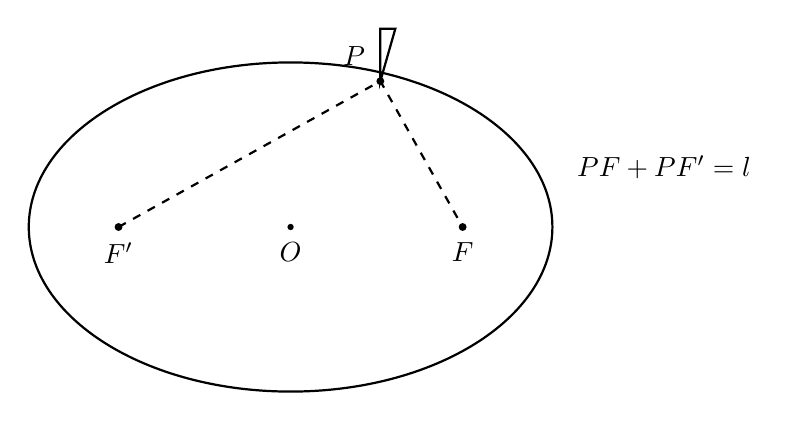
\begin{tikzpicture}[>=stealth, scale=0.95]
  % Draw ellipse
  \draw[thick] (0,0) ellipse (3.5cm and 2.2cm);
  % Foci
  \coordinate (F1) at (-2.3,0);
  \coordinate (F2) at (2.3,0);
  \coordinate (P) at (1.2, 1.95);
  \coordinate (O) at (0,0);
  \fill (O) circle (1.2pt) node[below=2pt] {$O$};
  \fill (F1) circle (1.5pt) node[below=2pt] {$F'$};
  \fill (F2) circle (1.5pt) node[below=2pt] {$F$};
  \fill (P) circle (1.5pt) node[above left=2pt] {$P$};
  % Strings
  \draw[thick, dashed] (F1) -- (P) -- (F2);
  % Pencil tip sketch
  \draw[thick] (P) -- ++(0.2, 0.7) -- ++(-0.2, 0) -- cycle;
  % Condition label on the right
  \node[right] at (3.7, 0.8) {$PF + PF' = l$};
\end{tikzpicture}
\caption{橢圓的繪法}
\label{fig:b4-3-1}
\end{figure}

\begin{definition*}
平面上到兩固定點 $F$ 與 $F'$ 之距離和為一定長 $l$ 的點所組成的曲線，稱為\textbf{橢圓}，其中 $l > \overline{FF'}$，通常 $F$ 與 $F'$ 稱為橢圓的兩個\textbf{焦點}．線段 $FF'$ 之中點 $O$ 稱為\textbf{橢圓中心}．

換句話說：對平面上一曲線 $\Gamma_-$，如存在兩點 $F$ 及 $F'$，一方面（不一定相異）使這曲線 $\Gamma_-$ 上的任一點 $P$ 滿足
\begin{equation}
PF + PF' = \text{定長} \label{eq:b4-3-1-1}
\end{equation}
另一方面使任何滿足上式的點 $P$ 都在這曲線 $\Gamma_-$ 上，則這曲線 $\Gamma_-$ 稱為一個橢圓．$PF$ 與 $PF'$ 稱為過 $P$ 的兩個\textbf{焦半徑}．
\end{definition*}

從這個定義，我們注意到橢圓由 $F, F'$ 之位置及尺長 $l$ 完全決定．若不計橢圓之位置，只計其形狀大小，則橢圓由長度 $\overline{FF'}$ 及 $l$ 完全決定．

這一性質很顯然是負類錐線的一個特徵性質，因此負類錐線都是橢圓，至於它的反命題將在乙段說明．設 $\Gamma_-$ 為一已知橢圓，$F, F'$ 為兩焦點，$O$ 為其中心，今連結 $FF'$，得一直線 $L$，在 $L$ 上 $F$ 與 $F'$ 按序分居於 $O$ 的右與左兩側，如圖 1-2．設 $A$ 點為這橢圓 $\Gamma_-$ 的一個交點而以 $a$ 表 $O$ 到 $A$ 的距離 $OA$．先考慮 $A$ 與 $F$ 同在 $O$ 的右側這一情況，此時 $A$ 更落在 $F$ 的右側〔不然，則 $AF + AF' = FF' < l$ 不符合 $A$ 在 $\Gamma_-$ 上的假定〕．

\begin{figure}[htbp]
\centering
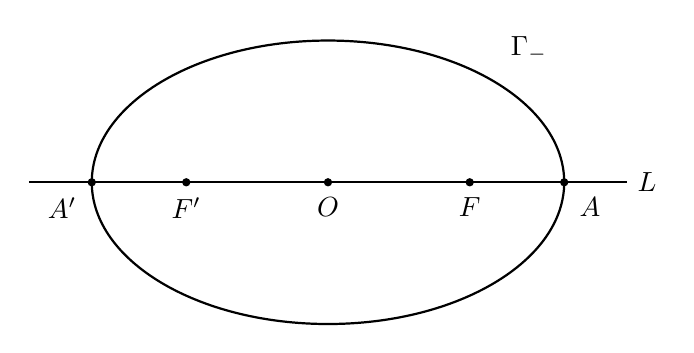
\begin{tikzpicture}[>=stealth, scale=1.0]
  \draw[thick] (-3.8,0) -- (3.8,0) node[right] {$L$};
  \coordinate (O) at (0,0);
  \coordinate (F1) at (-1.8,0);
  \coordinate (F2) at (1.8,0);
  \coordinate (A1) at (-3.0,0);
  \coordinate (A2) at (3.0,0);
  \fill (O) circle (1.5pt) node[below=2pt] {$O$};
  \fill (F1) circle (1.5pt) node[below=2pt] {$F'$};
  \fill (F2) circle (1.5pt) node[below=2pt] {$F$};
  \fill (A1) circle (1.5pt) node[below left=2pt] {$A'$};
  \fill (A2) circle (1.5pt) node[below right=2pt] {$A$};
  \draw[thick] (0,0) ellipse (3.0cm and 1.8cm);
  \node[above right] at (2.2, 1.4) {$\Gamma_-$};
\end{tikzpicture}
\caption{橢圓頂點與焦點}
\label{fig:b4-3-2}
\end{figure}

今
\begin{align*}
l &= AF + AF' \\
  &= AF + (AO + OF') \quad \text{〔因 $A$ 與 $F'$ 分居於 $O$ 的兩側〕} \\
  &= (AF + FO) + AO \quad \text{〔因 $OF' = FO$〕} \\
  &= AO + AO = 2a \quad \text{〔因 $A$ 與 $O$ 分居於 $F$ 之兩側〕}
\end{align*}
同理，若 $A'$ 與 $F'$ 同在 $O$ 的左側，亦得 $l = 2a$，故橢圓 $\Gamma_-$ 與 $L$ 確有兩交點 $A, A'$ 分別處於 $F$ 的右側與 $F'$ 的左側，且 $A$ 與 $A'$ 到 $O$ 的距離等長，其值為 $a$．

當我們想取一直角座標系使橢圓的方程式成一最簡潔的形式時，上述的討論自然也提示我們選線段 $F'F$ 的中點 $O$ 為原點，而選直線 $F'F$ 為 $x$ 軸，對於這樣的一個正交座標系 $(O; X, Y)$，我們可取兩實數 $a$ 與 $c \ge 0$，使 $F, F', A, A'$ 各點座標為
\[ A'(-a,0), \quad F'(-c,0), \quad F(c,0), \quad A(a,0) \]
注意：因 $l > \overline{FF'}$，而 $l = 2a, \overline{FF'} = 2c$，故 $a > c$．

\begin{definition*}
線段 $AA'$ 稱為橢圓之\textbf{長軸}，其長之半 $a = \frac{1}{2}\overline{AA'}$ 稱為\textbf{長軸半長}，橢圓 $\Gamma_-$ 的\textbf{離心率} $e$ 為
\[ e = \frac{\overline{FF'}}{\overline{AA'}} = \frac{c}{a} \]
卽知 $0 \le e < 1$\phantomsection\label{note:b4-ch3-e-circle}\footnote{〔原書註〕$e=0$ 表示焦距 $c=0$，即二焦點重合，此時 $a=b=\frac{1}{2}l$ 而圖形為一圓．圓是橢圓的特異情形，稍後將特別討論圓．}．
\end{definition*}

\begin{figure}[htbp]
\centering
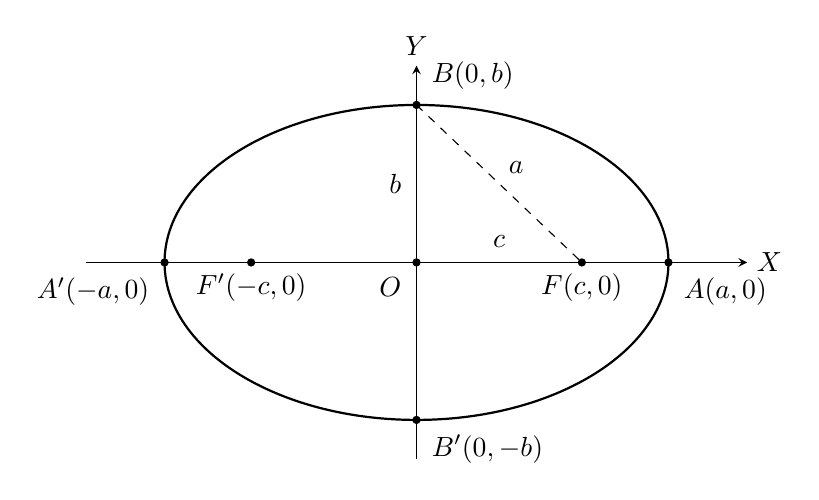
\begin{tikzpicture}[>=stealth, scale=1.0]
  \draw[->] (-4.2,0) -- (4.2,0) node[right] {$X$};
  \draw[->] (0,-2.5) -- (0,2.5) node[above] {$Y$};
  \draw[thick] (0,0) ellipse (3.2cm and 2.0cm);
  \coordinate (O) at (0,0);
  \coordinate (F1) at (-2.1,0);
  \coordinate (F2) at (2.1,0);
  \coordinate (A1) at (-3.2,0);
  \coordinate (A2) at (3.2,0);
  \coordinate (B1) at (0,2.0);
  \coordinate (B2) at (0,-2.0);
  \fill (O) circle (1.5pt) node[below left=2pt] {$O$};
  \fill (F1) circle (1.5pt) node[below=3pt, fill=white, inner sep=1pt] {$F'(-c,0)$};
  \fill (F2) circle (1.5pt) node[below=3pt, fill=white, inner sep=1pt] {$F(c,0)$};
  \fill (A1) circle (1.5pt) node[below left=2pt] {$A'(-a,0)$};
  \fill (A2) circle (1.5pt) node[below right=2pt] {$A(a,0)$};
  \fill (B1) circle (1.5pt) node[above right=2pt] {$B(0,b)$};
  \fill (B2) circle (1.5pt) node[below right=2pt] {$B'(0,-b)$};
  \draw[dashed] (B1) -- (F2) node[midway, above right] {$a$};
  \node[above=2pt] at (1.05, 0) {$c$};
  \node[left=2pt] at (0, 1.0) {$b$};
\end{tikzpicture}
\caption{橢圓與正交座標系}
\label{fig:b4-3-3}
\end{figure}

另一方面，設 $B(0,b)$ 為橢圓 $\Gamma_-$ 與 $Y$ 軸的交點，則 $BF + BF' = l = 2a$．但 $Y$ 軸為線段 $FF'$ 之中垂線故 $BF = BF' = a$，遂知
\[ b^2 = a^2 - c^2 \]
因此 $b = \sqrt{a^2 - c^2}$，亦卽橢圓 $\Gamma_-$ 截 $Y$ 軸於兩點 $B(0,b)$ 與 $B'(0,-b)$．線段 $BB'$ 稱為橢圓的\textbf{短軸}，$b$ 稱為\textbf{短軸半長}，$A, A', B, B'$ 稱為橢圓的\textbf{頂點}．

這時候我們已可由這四點 $A, A', B, B'$ 得到了「由到兩定點距離和為定長之點」這一軌跡（卽所謂橢圓）的大體輪廓，進一步，我們要準確地以方程式來表示這一軌跡．

\begin{proposition}
給定一橢圓 $\Gamma_-$ 可取一正交座標系 $(O; \mathbf{e}_1, \mathbf{e}_2)$ 使橢圓中心為原點 $(0,0)$，兩焦點為 $F(c,0), F'(-c,0)$，長軸長為 $2a$，則橢圓的方程式為
\begin{equation}
\Gamma_- : \frac{x^2}{a^2} + \frac{y^2}{b^2} = 1 \label{eq:b4-3-1-2}
\end{equation}
其中 $b = \sqrt{a^2 - c^2}$．
\end{proposition}

\begin{figure}[htbp]
\centering
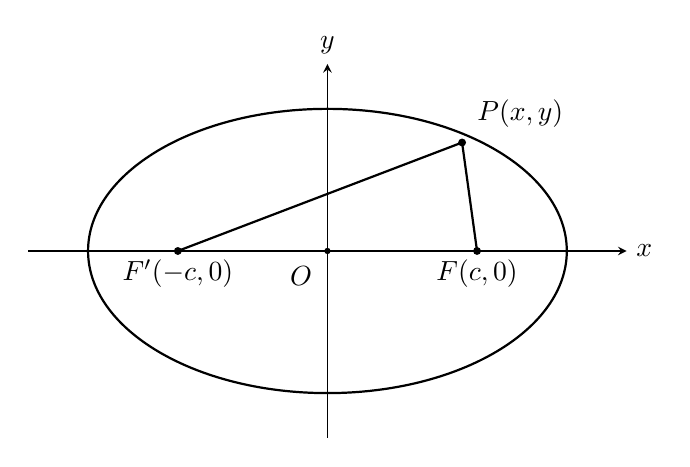
\begin{tikzpicture}[>=stealth, scale=0.95]
  \draw[->] (-4,0) -- (4,0) node[right] {$x$};
  \draw[->] (0,-2.5) -- (0,2.5) node[above] {$y$};
  \draw[thick] (0,0) ellipse (3.2cm and 1.9cm);
  \coordinate (O) at (0,0);
  \coordinate (F1) at (-2.0,0);
  \coordinate (F2) at (2.0,0);
  \coordinate (P) at (1.8, 1.45);
  \fill (O) circle (1.2pt) node[below left=2pt] {$O$};
  \fill (F1) circle (1.5pt) node[below=2pt, fill=white, inner sep=1pt] {$F'(-c,0)$};
  \fill (F2) circle (1.5pt) node[below=2pt, fill=white, inner sep=1pt] {$F(c,0)$};
  \fill (P) circle (1.5pt) node[above right=2pt] {$P(x,y)$};
  \draw[thick] (F1) -- (P) -- (F2);
\end{tikzpicture}
\caption{橢圓上一點與兩焦點}
\label{fig:b4-3-3prime}
\end{figure}

\begin{proof}
設 $P(x,y)$ 為 $\Gamma_-$ 上的一般點，則因 $PF + PF' = 2a$，推得
\begin{equation}
\sqrt{(x-c)^2 + y^2} + \sqrt{(x+c)^2 + y^2} = 2a \notag
\end{equation}
移項得
\[ \sqrt{(x-c)^2 + y^2} = 2a - \sqrt{(x+c)^2 + y^2} \]
兩端平方得
\[ (x-c)^2 + y^2 = 4a^2 - 4a\sqrt{(x+c)^2 + y^2} + (x+c)^2 + y^2 \]
稍加整理，得
\begin{equation}
a\sqrt{(x+c)^2 + y^2} = a^2 + cx \label{eq:b4-3-1-3}
\end{equation}
兩端再作平方：
\[ a^2[(x+c)^2 + y^2] = (a^2 + cx)^2 = a^4 + 2a^2cx + c^2x^2 \]
展開化簡：
\[ a^2x^2 + 2a^2cx + a^2c^2 + a^2y^2 = a^4 + 2a^2cx + c^2x^2 \]
\begin{equation}
(a^2 - c^2)x^2 + a^2y^2 = a^2(a^2 - c^2) \label{eq:b4-3-1-4}
\end{equation}
以 $b^2 = a^2 - c^2$ 代入得
\[ b^2x^2 + a^2y^2 = a^2b^2 \]
除以 $a^2b^2$：
\[ \frac{x^2}{a^2} + \frac{y^2}{b^2} = 1 \]
\end{proof}

取適當的正交座標系，橢圓這一看似複雜的曲線竟以 \eqref{eq:b4-3-1-2} 式這簡潔的形式出現，這個 \eqref{eq:b4-3-1-2} 式我們就稱為橢圓的\textbf{標準式}．

注意在 \eqref{eq:b4-3-1-2} 式的導引過程中，作了兩次平方，照理可能會產生很多不見得仍滿足原來關係式
\[ PF + PF' = 2a \]
的點 $(x,y)$．第一次作平方後實際上考慮的已經是滿足
\[ \pm PF \pm PF' = 2a \]
的所有點 $(x,y)$ 了．第二次再作平方，所考慮的點更增多到所有滿足
\[ \pm PF \pm PF' = \pm 2a \]
的 $(x,y)$，其中左右兩端的 $\pm$ 號可以分配為 $(+,+), (+,-), (-,+), (-,-)$ 等四種可能．而我們的式子只不過是第二種 $(+,-)$ 的情形：
今分述其餘三種情形如下：
\begin{enumerate}[(i)]
  \item $(-,+)$ 的情形，因 $2a > 0$ 故不可能發生．
  \item $(+,+)$ 與 $(-,-)$ 的情形，其實可合寫為 $|PF - PF'| = 2a > 2c = FF'$，上式表示三角形 $\triangle PFF'$ 兩邊之差會大於第三邊，此為不可能故不致產生這樣的 $P(x,y)$ 點．
\end{enumerate}
故平方過程所可能引進的多餘軌跡其實均不存在，換言之，方程式 \eqref{eq:b4-3-1-2} 的實數解恰好就是橢圓上的點．

標準式 \eqref{eq:b4-3-1-2} 雖然看似代表某一種特殊的橢圓，但是如果我們不計較橢圓的位置，只考慮它的形狀與大小，標準式這種形式的方程式實際上卻是描寫了所有的橢圓．

\begin{example}
如橢圓中心不在已給自然座標系的原點，而在點 $(1,1)$，兩焦點座標分別為 $F=(2,1), F'=(0,1)$，長軸半長為 2，則此橢圓的方程式為何？

\begin{figure}[htbp]
\centering
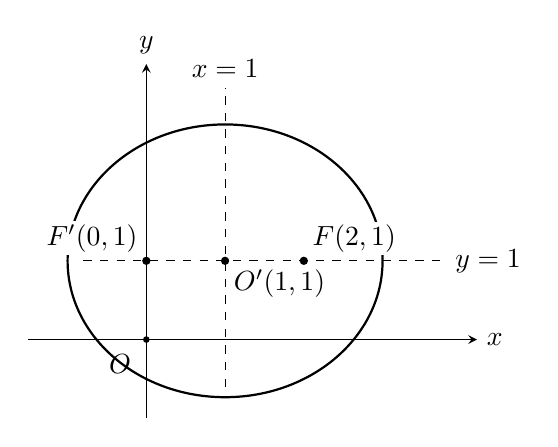
\begin{tikzpicture}[>=stealth, scale=1.0]
  \draw[->] (-1.5,0) -- (4.2,0) node[right] {$x$};
  \draw[->] (0,-1) -- (0,3.5) node[above] {$y$};
  \coordinate (O) at (0,0);
  \coordinate (O1) at (1,1);
  \coordinate (F1) at (0,1);
  \coordinate (F2) at (2,1);
  \draw[dashed] (-0.8,1) -- (3.8,1) node[right] {$y=1$};
  \draw[dashed] (1,-0.6) -- (1,3.2) node[above] {$x=1$};
  \draw[thick] (1,1) ellipse (2.0cm and 1.732cm);
  \fill (O) circle (1.2pt) node[below left=2pt] {$O$};
  \fill (O1) circle (1.5pt) node[below right=2pt, fill=white, inner sep=1pt] {$O'(1,1)$};
  \fill (F1) circle (1.5pt) node[above left=2pt, fill=white, inner sep=1pt] {$F'(0,1)$};
  \fill (F2) circle (1.5pt) node[above right=2pt, fill=white, inner sep=1pt] {$F(2,1)$};
\end{tikzpicture}
\caption{中心在 $(1,1)$ 的橢圓}
\label{fig:b4-3-4}
\end{figure}

\textbf{解 1}\quad 設 $P(x,y)$ 為 $\Gamma_-$ 上的一般點，則由橢圓定義：
\[ PF + PF' = 2 \times 2 = 4 \]
卽
\[ \sqrt{(x-2)^2 + (y-1)^2} + \sqrt{x^2 + (y-1)^2} = 4 \]
兩端平方，得
\[ \sqrt{x^2 + (y-1)^2} = 2 + \frac{1}{2}x \]
再平方得
\[ 4[x^2 + (y-1)^2] = (4 + x)^2 = 16 + 8x + x^2 \]
配方整理得：
\[ 3(x-1)^2 + 4(y-1)^2 = 12 \]
注意：此橢圓的長軸在 $y-1=0$ 上，平行於 $X$ 軸，短軸則在 $x-1=0$，且 $a=2, c=1$，故 $b^2 = a^2 - c^2 = 4-1 = 3$，故上式的形式，其實就是
\[ \frac{(x-1)^2}{4} + \frac{(y-1)^2}{3} = 1 \]

\textbf{解 2}\quad 取一正交座標系 $S$ 使 $O'=(1,1)$ 為 $S$ 的原點，原基底為 $S$ 的基底，則 $F=(2,1) = (1,0)_S$，$F'=(0,1) = (-1,0)_S$．因 $c = \overline{O'F} = 1, a = 2$，故 $b = \sqrt{3}$；故可得相關於 $S$ 的橢圓表示式為
\[ \frac{X^2}{4} + \frac{Y^2}{3} = 1 \]
因新舊座標的關係為：$X = x-1, Y = y-1$，故根據原自然座標系橢圓方程式為：
\[ \frac{(x-1)^2}{4} + \frac{(y-1)^2}{3} = 1 \]
此與解 1 所得的形式相同．我們有時也稱此類的形式為\textbf{準標準形}，因為可以從此形式中，直截看出圖形為橢圓，且定出中心位置及長短軸的大小．（注意標準式中無 $xy$ 項）
\end{example}

\begin{exercise}
\begin{enumerate}[(i)]
  \item 設橢圓中心為 $(1,1)$，兩焦點座標分別為 $F=(1,0), F'=(1,2)$，長軸長為 4，試求此橢圓方程式．如何寫成標準式？
  \item 當 $b > a > 0$ 時，$\frac{x^2}{a^2} + \frac{y^2}{b^2} = 1$ 之圖形為何？焦點位置為何？
  \item 試證中心在 $(h,k)$，兩焦點為 $F(h+c, k), F'(h-c, k)$，半長軸為 $a$ 的橢圓方程式為
  \[ \frac{(x-h)^2}{a^2} + \frac{(y-k)^2}{a^2 - c^2} = 1 \]
  \item 設 $F=(1,1), F'=(0,-1)$，$PF + PF' = 3$，試求滿足上述條件的點 $P$ 所形成的橢圓方程式，並注意所得的方程式能否寫成前文所述的準標準型？（例如用配方法）（提示：在自然座標系中不可能，到第四章我們將講述如何用固有值的方法，求得一新正交座標系而將橢圓的方程式化成標準型．）
\end{enumerate}
\end{exercise}

\subsubsection*{乙、橢圓的形狀}

講到橢圓的形狀能否加以「數量化」，亦卽能否以幾個數量來決定它的形狀？這便觸及數學的一個主要精神．標準式 \eqref{eq:b4-3-1-2} 其實已相當程度告訴了我們 $a$ 與 $b$ 是怎樣的兩個數量，但讓我們更原始地來看這一問題．在前面定義過橢圓之後，我們馬上提出它可由 $F, F'$ 的位置及定長 $l$ 決定．現在當我們不計較橢圓位置，而只看它的形狀時，決定的因素實際上便只是長度 $\overline{FF'}$ 與 $l$ 而已，但
\[ c = \frac{1}{2}\overline{FF'}, \quad a = \frac{1}{2}l \]
故決定的因素亦可視為 $a$ 與 $c$，$\{a, c\}$ 二值可作為決定橢圓的一組資料．更進一層，因離心率 $e = \frac{c}{a}$，故若知 $e$ 與 $a$，則知 $c = ae$，便知橢圓之形狀，卽二數 $\{a, e\}$ 亦為決定橢圓的一組資料．若 $e \neq 0$ 則 $\{a, e\}$ 與 $\{a, c\}$ 這兩組資料相互決定，我們稱 $\{a, e\}$ 與 $\{a, c\}$ 為等價的資料．

就幾何意義來說，我們較易用離心率 $e$ 與長軸長 $a$ 來看出橢圓形狀的變化，離心率 $e$ 決定扁的程度：固定 $a$ 則 $e$ 越大橢圓越扁；而 $a$ 決定其大小：固定 $e$ 則當 $a$ 增加，橢圓亦隨比例相似地擴大（見圖 1-5）．

\begin{figure}[htbp]
\centering
\begin{tikzpicture}[>=stealth, scale=0.85]
  % Left: a fixed = 4, e varies
  \begin{scope}[xshift=-4.5cm]
    \node[anchor=west] at (-4.2, 4.3) {\small ($a$ 固定為 4)};
    \draw[->] (-4.5,0) -- (4.5,0) node[right] {$x$};
    \draw[->] (0,-4.0) -- (0,4.2) node[above] {$y$};
    \draw[thick] (0,0) ellipse (4cm and 3.66cm); % e=0.4
    \node[above=1pt, fill=white, inner sep=1pt] at (0, 3.66) {\small $e=0.4$};
    \draw[thick, dashed] (0,0) ellipse (4cm and 2.85cm); % e=0.7
    \node[above=1pt, fill=white, inner sep=1pt] at (0, 2.85) {\small $e=0.7$};
    \draw[thick, dotted] (0,0) ellipse (4cm and 1.74cm); % e=0.9
    \node[above=1pt, fill=white, inner sep=1pt] at (0, 1.74) {\small $e=0.9$};
  \end{scope}
  % Right: e fixed = 0.8, a varies
  \begin{scope}[xshift=4.5cm]
    \node[anchor=west] at (-4.2, 4.3) {\small ($e$ 固定為 0.8)};
    \draw[->] (-4.5,0) -- (4.5,0) node[right] {$x$};
    \draw[->] (0,-3.2) -- (0,3.5) node[above] {$y$};
    % e=0.8, b/a = sqrt(1-0.64) = 0.6
    \draw[thick] (0,0) ellipse (1.8cm and 1.08cm); % a=3
    \node[above=1pt, fill=white, inner sep=1pt] at (0, 1.08) {\small $a=3$};
    \draw[thick, dashed] (0,0) ellipse (3.0cm and 1.8cm); % a=5
    \node[above=1pt, fill=white, inner sep=1pt] at (0, 1.8) {\small $a=5$};
    \draw[thick, dotted] (0,0) ellipse (4.2cm and 2.52cm); % a=7
    \node[above=1pt, fill=white, inner sep=1pt] at (0, 2.52) {\small $a=7$};
  \end{scope}
\end{tikzpicture}
\caption{離心率與長軸對橢圓形狀的影響}
\label{fig:b4-3-5}
\end{figure}

\begin{example}
設二橢圓 $\Gamma_-$ 與 $\Gamma_-'$ 各由 $\{e, a\}$ 與 $\{e, a'\}$ 決定，其中 $e$ 為離心率，$a, a'$ 為長軸半長，試證 $\Gamma_-$ 與 $\Gamma_-'$ 相似，亦卽若取 $\lambda = \frac{a'}{a}$，則在平面上作適當之剛性運動使二橢圓之中心與對稱軸重合後，有
\[ (x,y) \in \Gamma_- \iff (\lambda x, \lambda y) \in \Gamma_-' \]

\begin{proof}
因形狀大小與位置無關，可將二橢圓中心重合，取為原點，且長軸均重合於 $X$ 軸，則二橢圓之標準式各為
\[ \Gamma_- : \frac{x^2}{a^2} + \frac{y^2}{b^2} = 1, \quad \text{其中 } b = a\sqrt{1-e^2} \]
\[ \Gamma_-' : \frac{x^2}{a'^2} + \frac{y^2}{b'^2} = 1, \quad \text{其中 } b' = a'\sqrt{1-e^2} \]
若設 $\lambda = \frac{a'}{a}$，則 $a' = \lambda a, b' = \lambda b$，將 $(\lambda x, \lambda y)$ 代入 $\Gamma_-'$ 得
\[ \frac{(\lambda x)^2}{(\lambda a)^2} + \frac{(\lambda y)^2}{(\lambda b)^2} = \frac{\lambda^2 x^2}{\lambda^2 a^2} + \frac{\lambda^2 y^2}{\lambda^2 b^2} = \frac{x^2}{a^2} + \frac{y^2}{b^2} = 1 \]
故 $(\lambda x, \lambda y) \in \Gamma_-' \iff (x,y) \in \Gamma_-$，我們稱 $\Gamma_-'$ 為 $\Gamma_-$ 的 $\lambda$ 倍放大．
\end{proof}
\end{example}

\begin{example}[橢圓之伸縮作圖]
求作 $\frac{x^2}{16} + \frac{y^2}{4} = 1$ 之圖形．

\textbf{解}\quad 將方程式兩邊乘以 4，使 $y^2$ 項的係數為 1，則方程式變成
\begin{equation}
\frac{x^2}{4} + y^2 = 4 \quad \text{卽} \quad \left(\frac{x}{2}\right)^2 + y^2 = 2^2 \label{eq:b4-3-ex3}
\end{equation}
若設 $x' = \frac{x}{2}, y' = y$，則上式可寫成
\[ x'^2 + y'^2 = 2^2 \]
這對 $(x', y')$ 而言為以原點為心，半徑等於 2 之圓（見圖 1-6a）．因 $x = 2x'$，故將此圓圖形的橫軸方向放大 2 倍，卽得原橢圓之圖形（見圖 1-6b）．

\begin{figure}[htbp]
\centering
\begin{tikzpicture}[>=stealth, scale=0.85]
  % 1-6a
  \begin{scope}[xshift=-3.5cm]
    \draw[->] (-3,0) -- (3,0) node[right] {$x'$};
    \draw[->] (0,-3) -- (0,3) node[above] {$y'$};
    \draw[thick] (0,0) circle (2cm);
    \node[below left] at (0,0) {$O$};
    \node[below] at (2,0) {$2$};
    \node[left] at (0,2) {$2$};
    \node at (0, -3.3) {圖 1-6a};
  \end{scope}
  % 1-6b
  \begin{scope}[xshift=3.5cm]
    \draw[->] (-4.5,0) -- (4.5,0) node[right] {$x$};
    \draw[->] (0,-3) -- (0,3) node[above] {$y$};
    \draw[thick] (0,0) ellipse (4cm and 2cm);
    \node[below left] at (0,0) {$O$};
    \node[below] at (4,0) {$4$};
    \node[left] at (0,2) {$2$};
    \node at (0, -3.3) {圖 1-6b};
  \end{scope}
\end{tikzpicture}
\caption{橢圓之伸縮作圖法}
\label{fig:b4-3-6}
\end{figure}
\end{example}

\begin{exercise}
仿上述論例求作 $\frac{x^2}{9} + \frac{y^2}{25} = 1$ 之圖形．
\end{exercise}

\begin{example}
各行星相對於太陽的軌道為橢圓，其離心率及平均軌道半徑列表如下：
\begin{center}
\begin{tabular}{|c|c|c|c|}
\hline
行星 & 離心率 $e$ & 平均軌道半徑（$\text{AU}$） & 週期（日） \\ \hline
水星 & 0.206 & 0.389 & 87.77 \\ \hline
金星 & 0.007 & 0.724 & 224.70 \\ \hline
地球 & 0.017 & 1.000 & 365.25 \\ \hline
火星 & 0.093 & 1.524 & 686.98 \\ \hline
木星 & 0.048 & 5.200 & 4332.62 \\ \hline
土星 & 0.056 & 9.510 & 10789.20 \\ \hline
天王星 & 0.047 & 19.191 & 30685.93 \\ \hline
\end{tabular}
\end{center}
其中所謂平均軌道半徑為行星至太陽最遠與最近距離之平均值，這平均軌道半徑也就是長軸半長 $a$．（我們取地球至太陽的平均軌道半徑為一天文單位 astronomical unit，簡記以 $\text{AU}$．）

設行星的橢圓軌道方程式為：$\frac{x^2}{a^2} + \frac{y^2}{b^2} = 1$，式中太陽在 $F(c,0)$ 處，最近點與最遠點分別為 $A, A'$，則 $A=(a,0), A'=(-a,0)$，故平均軌道半徑應為 $(a-c)$ 與 $(a+c)$ 之平均值，卽等於 $a$．今取火星為例，其離心率為 $e = 0.093$，平均軌道半徑 $a = 1.524\text{ AU}$，則
\[ c = ae = 1.524 \times 0.093 = 0.141732\text{ AU} \]
則最近與最遠距離分別為
\[ a - c = 1.382268\text{ AU}, \qquad a + c = 1.665732\text{ AU} \]

\begin{figure}[htbp]
\centering
\begin{tikzpicture}[>=stealth, scale=1.0]
  \draw[thick] (0,0) ellipse (3.5cm and 2.5cm);
  \coordinate (Sun) at (1.2,0);
  \coordinate (A) at (3.5,0);
  \coordinate (Aprime) at (-3.5,0);
  \fill[orange!90!black] (Sun) circle (3.5pt) node[below=4pt] {太陽 $F$};
  \fill (A) circle (2pt) node[right=3pt] {近日點（行星）};
  \fill (Aprime) circle (2pt) node[left=3pt] {遠日點};
  % Dimension lines above
  \draw[<->] ($(Sun)+(0,0.8)$) -- ($(A)+(0,0.8)$) node[midway, fill=white, inner sep=1pt] {$a-c$};
  \draw[<->] ($(Aprime)+(0,0.8)$) -- ($(Sun)+(0,0.8)$) node[midway, fill=white, inner sep=1pt] {$a+c$};
  \draw[dotted] (Sun) -- ($(Sun)+(0,0.8)$);
  \draw[dotted] (A) -- ($(A)+(0,0.8)$);
  \draw[dotted] (Aprime) -- ($(Aprime)+(0,0.8)$);
\end{tikzpicture}
\caption{行星繞日橢圓軌道}
\label{fig:b4-3-7}
\end{figure}
\end{example}

\begin{exercise}
何以行星到太陽的最近點與最遠點分別為其橢圓軌道之長軸上的兩頂點？九大行星中哪一行星軌道最扁，次扁？哪一行星軌道最近於正圓？
\end{exercise}

\begin{exercise}
仿論例 3 作圖法，描繪水星、土星、海王星之軌道．
\end{exercise}

\begin{exercise}
\begin{enumerate}[(i)]
  \item 固定 $a=5$，試大略繪出 $e=0.4, 0.7, 0.9$ 的橢圓曲線．
  \item 固定 $a=2$，而讓 $e$ 變動寫出相應的橢圓系，卽一系列的橢圓的方程式，並作圖表明其隨 $e$ 變化的情形．〔提示：在 $\Gamma_- : \frac{x^2}{a^2} + \frac{y^2}{b^2} = 1$ 中，$b^2 = a^2(1-e^2)$〕
  \item 已知 $e = \frac{3}{5}$，試大略繪出半長軸為 $5, 7, 10$ 時的橢圓曲線．
  \item 固定 $e = \frac{1}{2}$ 而讓 $a$ 變動，寫出其相應的橢圓系方程式，並作圖表明其隨 $a$ 變化的變化．
  \item 固定 $c=1$，而讓 $a$ 變動寫出相應的橢圓方程式，當 $a$ 趨於 $c$ 時，橢圓的極限位置為何？
\end{enumerate}
\end{exercise}

利用離心率與長軸半長，我們便可以說明一項重要事實．

\begin{proposition}
橢圓其實就是負類錐線．
\end{proposition}

\begin{proof}[說明]
「兩焦半徑之和為定長」據定義便是橢圓，而負類錐線在第二章中已證得有此特徵性質，故負類錐線必為一橢圓．反過來給定一橢圓 $\Gamma_-$ 設其離心率為 $e_0$，長軸半長為 $a_0$，我們要找出一負類錐線 $\Gamma$ 使兩曲線 $\Gamma_-$ 與 $\Gamma$ 的形狀一致：
\begin{enumerate}[(i)]
  \item 取一固定圓錐 $\Omega$，其頂角 $\alpha$，設一平面 $\pi$ 在 $\Omega$ 上的截角為 $\theta$ ($0 < \theta < \alpha'$)，在第二章已導得截痕 $\Gamma$ 之離心率為
  \[ e = \frac{\sin\theta}{\sin\alpha'} \]
  現在取截角 $\theta$ 為 $\theta_0$ 使 $\sin\theta_0 = e_0 \sin\alpha'$．這是辦得到的，道理是：$0 \le e_0 < 1$ 且當 $\theta$ 從 $0$ 變化到 $\alpha'$ 時，$\frac{\sin\theta}{\sin\alpha'}$ 之值亦從 $0$ 變化到 $1$，故必有某 $\theta_0$ 使比值等於已給的 $e_0$．這樣相應於截角為 $\theta_0$ 時的負類錐線 $\Gamma$ 的離心率便為 $e_0$．
  \item 所剩的便是調整 $\Gamma$ 的大小．將 $\Gamma$ 所在的截面 $\pi$ 上下平行移動（見圖 1-8），藉以調整其長軸，則因這樣的移動，使其長軸半長範圍從 $0$ 伸向 $\infty$，故必得一平面 $\pi$ 其長軸之半長為 $a_0$．
\end{enumerate}
對於這樣取得的 $\pi$，其截在 $\Omega$ 上的錐線因已知為一橢圓，且其離心率及其長軸半長皆與已給定的橢圓 $\Gamma_-$ 的離心率 $e_0$ 與長軸半長 $a_0$ 吻合，卽 $\Gamma_-$ 成為一負類錐線．
\end{proof}

\begin{figure}[htbp]
\centering
\begin{tikzpicture}[>=stealth, scale=0.9]
  % Cone
  \coordinate (V) at (0,2.5);
  \draw[thick] (-2.5,-3) -- (V) node[above] {$K$} -- (2.5,-3);
  \draw[dashed] (0,2.5) -- (0,-3.2);
  % Elliptic sections parallel
  \draw[thick, fill=blue!5, fill opacity=0.3, rotate around={-25:(0,0.8)}] (0,0.8) ellipse (1.1cm and 0.45cm);
  \draw[thick, fill=blue!10, fill opacity=0.3, rotate around={-25:(0,-1.2)}] (0,-1.2) ellipse (2.1cm and 0.85cm);
  \node[right] at (1.1, 0.4) {$\pi$};
  \node[right] at (2.0, -1.6) {$\pi'$};
  \draw[->, thick] (1.3, -0.6) -- (1.3, 0.4) node[midway, right] {平行移動};
\end{tikzpicture}
\caption{圓錐截面之平行移動}
\label{fig:b4-3-8}
\end{figure}

從這一事實，我們更能把負類錐線所有已知的性質，都搬過來給橢圓．例如，根據準線觀點，那時已證得定理 I，現在我們也得到：

\begin{theorem}
給定一橢圓
\[ \Gamma_- : \frac{x^2}{a^2} + \frac{y^2}{b^2} = 1 \qquad (a > b > 0) \]
則存在兩直線（稱為橢圓 $\Gamma_-$ 的二準線）
\[ p: x = \frac{a^2}{c}, \qquad p': x = -\frac{a^2}{c} \]
使 $\Gamma_-$ 上任意 $P(x,y)$ 到焦點距離 $PF$（或 $PF'$）與到 $p$（或 $p'$）的距離 $PT$（或 $PT'$）為一定比，且這定比等於 $\Gamma_-$ 的離心率，亦卽
\begin{equation}
\frac{PF}{PT} = \frac{PF'}{PT'} = e \label{eq:b4-3-1-5}
\end{equation}
\end{theorem}

\subsubsection*{丙、準線觀點的再證明}

我們不妨在平面上利用座標幾何的方法，將上述的定理 I 重作證明如下：

\begin{figure}[htbp]
\centering
\begin{tikzpicture}[>=stealth, scale=1.0]
  \draw[->] (-4.5,0) -- (4.5,0) node[right] {$x$};
  \draw[->] (0,-2.5) -- (0,2.5) node[above] {$y$};
  \draw[thick] (0,0) ellipse (3.0cm and 1.8cm);
  \coordinate (O) at (0,0);
  \coordinate (F1) at (-1.8,0);
  \coordinate (F2) at (1.8,0);
  \coordinate (P) at (1.5, 1.56);
  \coordinate (T) at (3.8, 1.56);
  % Directrices
  \draw[thick, dashed] (3.8,-2.5) -- (3.8,2.5) node[above, fill=white, inner sep=1pt] {$p: x = \frac{a^2}{c}$};
  \draw[thick, dashed] (-3.8,-2.5) -- (-3.8,2.5) node[above, fill=white, inner sep=1pt] {$p': x = -\frac{a^2}{c}$};
  \fill (O) circle (1.2pt) node[below left=2pt] {$O$};
  \fill (F1) circle (1.5pt) node[below=2pt, fill=white, inner sep=1pt] {$F'(-c,0)$};
  \fill (F2) circle (1.5pt) node[below=2pt, fill=white, inner sep=1pt] {$F(c,0)$};
  \fill (P) circle (1.5pt) node[above left=2pt] {$P(x,y)$};
  \fill (T) circle (1.5pt) node[above right=2pt] {$T$};
  \draw[thick] (F2) -- (P);
  \draw[thick] (P) -- (T);
  % Right angle mark at T
  \draw ($(T)+(-0.2,0)$) |- ($(T)+(0,-0.2)$);
\end{tikzpicture}
\caption{橢圓與準線}
\label{fig:b4-3-9}
\end{figure}

\begin{proof}
設 $P(x,y)$ 為橢圓 $\Gamma_- : \frac{x^2}{a^2} + \frac{y^2}{b^2} = 1$ 上一點，則
\begin{equation}
y^2 = b^2\left(1 - \frac{x^2}{a^2}\right) = (a^2 - c^2)\left(1 - \frac{x^2}{a^2}\right) \label{eq:b4-3-1-6}
\end{equation}
而 $P$ 到 $p: x = \frac{a^2}{c}$ 的距離為
\[ PT = \left|\frac{a^2}{c} - x\right| = \frac{a^2}{c} - x \quad \left(\text{因 } x \le a < \frac{a^2}{c}\right) \]
將 \eqref{eq:b4-3-1-6} 代入 $PF^2 = (x-c)^2 + y^2$ 中得
\begin{align*}
PF^2 &= (x-c)^2 + (a^2 - c^2)\left(1 - \frac{x^2}{a^2}\right) \\
     &= x^2 - 2cx + c^2 + a^2 - c^2 - x^2 + \frac{c^2}{a^2}x^2 \\
     &= a^2 - 2cx + \frac{c^2}{a^2}x^2 = \left(a - \frac{c}{a}x\right)^2
\end{align*}
故
\[ PF = a - \frac{c}{a}x = \frac{c}{a}\left(\frac{a^2}{c} - x\right) = e \cdot PT \]
卽
\[ \frac{PF}{PT} = e \]
同理可證 $\frac{PF'}{PT'} = e$．
\end{proof}

\begin{exercise}
證明 $\frac{PF'}{PT'} = e$．
\end{exercise}

\begin{example}
試證論例 1 中橢圓的準線為 $x=5$ 及 $x=-3$（或 $x-1 = \pm 4$）．

\textbf{解 1}\quad 在座標系 $S(O'; X, Y)$ 中，橢圓方程式為
\[ \Gamma_- : \frac{X^2}{4} + \frac{Y^2}{3} = 1, \qquad a=2, b=\sqrt{3}, c=1 \]
由定理 I 知，兩直線 $p: X = \frac{a^2}{c} = 4, p': X = -\frac{a^2}{c} = -4$ 為 $\Gamma_-$ 相關於 $S$ 的準線方程式．此二直線相關於原座標系 $(O; x, y)$ 的方程式為：
\[ x-1 = 4 \implies x = 5, \qquad x-1 = -4 \implies x = -3 \]
卽為 $\Gamma_-$ 的準線．

\textbf{解 2}\quad 設 $P(x,y)$ 為 $\Gamma_-$ 上一點，則 $P$ 到 $p: x = 5$ 的距離為 $PT = |x - 5| = 5 - x$，由橢圓定義亦可直接推知 $\frac{PF}{PT} = e = \frac{1}{2}$．
\end{example}

\begin{exercise}
\begin{enumerate}[(i)]
  \item 設知一橢圓以 $(0,0)$ 為中心，準線分別為 $x = \pm 4$，而焦點為 $(-1,0)$ 與 $(1,0)$，試求此橢圓方程式．
  \item 當 $b > a > 0$，則 $\frac{x^2}{a^2} + \frac{y^2}{b^2} = 1$ 之準線為何？
\end{enumerate}
\end{exercise}

\subsubsection*{習題 III-1}

\begin{enumerate}
  \item 試求下列橢圓方程式，並作圖形：
  \begin{enumerate}[(i)]
    \item 焦點為 $(0, \pm 4)$，長軸兩端點為 $(0, \pm 5)$．
    \item 焦點為 $(0, \pm 3)$，準線為 $y = \pm \frac{25}{3}$．
    \item 焦點在 $x$ 軸上且其焦點與準線的距離為 7\phantomsection\label{note:b4-ch3-ex1-1-3}\footnote{【原書註記/校訂】：原書此題印作「且其 與準線的距離為 7」，脫漏「焦點」二字，茲予補正．}，離心率為 $\frac{3}{4}$，中心為原點．
    \item 焦點為 $(0, \pm 3)$，離心率為 $\frac{3}{5}$．
    \item[*] 中心為原點，軸為座標軸，通過 $(2,3)$ 及 $(-1,4)$．
  \end{enumerate}

  \item 試求橢圓之長短軸，中心位置，離心率，準線與焦距：
  \begin{enumerate}[(i)]
    \item $9x^2 + 4y^2 = 36$
    \item $8x^2 - 16x + 3y^2 = 31$
    \item $2x^2 = 1 - y^2$
    \item $3x^2 + 4y^2 - 16y = 20$
  \end{enumerate}
  （(ii), (iv) 用配方法）

  \item 長度 $l$ 的一線段 $AB$ 的兩端點，$A, B$ 分別在二垂直直線上移動，試求分 $\overline{AB}$ 為定比的點 $P$ 的軌跡．\\
  （提示：將此二垂直直線取為一直角座標系的二軸）

  \item 地球的軌道是以太陽為一焦點的橢圓，地球與太陽的最短和最長距離概分別均為 147.5 萬公里，152.5 萬公里．試求出地球軌道的長軸及離心率．

  \item[*] 橢圓方程式為 $\frac{x^2}{a^2} + \frac{y^2}{b^2} = 1$，$M(-4,\sqrt{2})$ 在其上，離心率為 $\frac{3}{4}$，求橢圓方程式，並求 $M$ 至二焦點的距離．

  \item 一橢圓的焦點間的距離等於不同軸的二頂點距離，求此橢圓離心率．

  \item 一長方形外切橢圓 $\frac{x^2}{a^2} + \frac{y^2}{b^2} = 1$ 於頂點，試求在長方形對角線上的弦長．

  \item 設有一橢圓中心在 $(2,2)$，其軸平行坐標軸，長軸為短軸之三倍，並通過 $(4,0)$，試求其方程式．

  \item 在一平面上取互相垂直二軸，以交點為中心，二定長 $a, b$ 為半徑做圓（$a > b$），由圓心畫任一半徑順次交兩圓於 $M$ 及 $N$，自 $M$ 做 $MR$ 平行縱軸，自 $N$ 做 $NS$ 平行橫軸，此二線相交于 $P$ 點．試證 $P$ 點在以 $2a$ 為長軸 $2\sqrt{a^2-b^2}$ 為焦距的橢圓上（見圖 1-10）．\\
  （提示：設 $\angle MOA = \phi$，求 $\sin\phi$ 與 $\cos\phi$，再利用畢氏定理）

\begin{figure}[htbp]
\centering
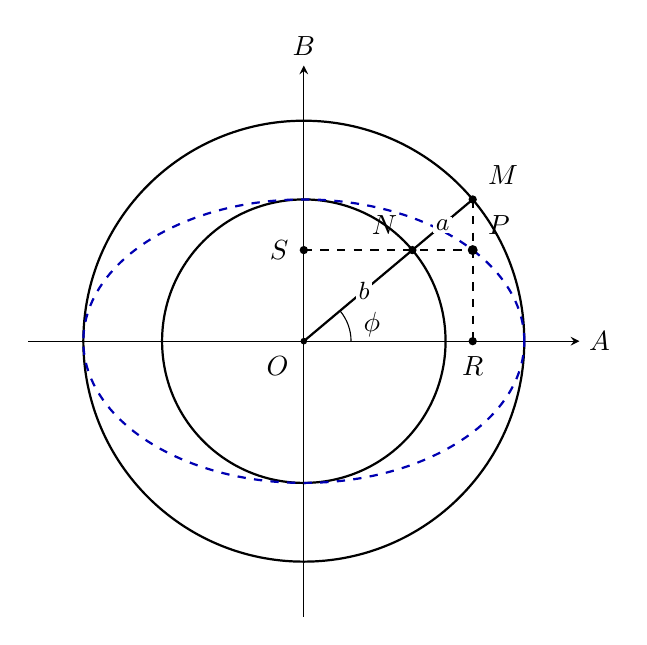
\begin{tikzpicture}[>=stealth, scale=1.0]
  \draw[->] (-3.5,0) -- (3.5,0) node[right] {$A$};
  \draw[->] (0,-3.5) -- (0,3.5) node[above] {$B$};
  \draw[thick] (0,0) circle (2.8cm); % radius a
  \draw[thick] (0,0) circle (1.8cm); % radius b
  \coordinate (O) at (0,0);
  % angle phi = 40 deg
  \coordinate (M) at (40:2.8);
  \coordinate (N) at (40:1.8);
  \coordinate (P) at ({2.8*cos(40)}, {1.8*sin(40)});
  \coordinate (R) at ({2.8*cos(40)}, 0);
  \coordinate (S) at (0, {1.8*sin(40)});
  % Dashed ellipse locus through P
  \draw[thick, dashed, blue!70!black] (0,0) ellipse (2.8cm and 1.8cm);
  \fill (O) circle (1.2pt) node[below left=2pt] {$O$};
  \fill (M) circle (1.5pt) node[above right=2pt] {$M$};
  \fill (N) circle (1.5pt) node[above left=2pt] {$N$};
  \fill (P) circle (1.8pt) node[above right=2pt] {$P$};
  \fill (R) circle (1.5pt) node[below=2pt] {$R$};
  \fill (S) circle (1.5pt) node[left=2pt] {$S$};
  % Radius ray OM
  \draw[thick] (O) -- (M);
  % Straight vertical line M-P-R
  \draw[thick, dashed] (M) -- (R);
  % Straight horizontal line S-N-P
  \draw[thick, dashed] (S) -- (P);
  % Angle arc
  \draw (0.6,0) arc (0:40:0.6) node[midway, right=2pt] {$\phi$};
  % Labels a and b along ray
  \node[fill=white, inner sep=1pt] at (40:1.0) {\small $b$};
  \node[fill=white, inner sep=1pt] at (40:2.3) {\small $a$};
\end{tikzpicture}
\caption{橢圓的輔助圓參數作圖法}
\label{fig:b4-3-10}
\end{figure}

\end{enumerate}

% =========================================================================
% § III-2 雙曲線
% =========================================================================
\subsection{雙曲線}
\label{sec:b4-3-2}

\subsubsection*{甲、雙曲線的定義與其標準式}

\begin{definition*}
平面上到兩個固定點 $F$ 與 $F'$ 之距離差為一定長 $l$ 的點所組成的曲線 $\Gamma_+$ 稱為\textbf{雙曲線}．

換句話說，對平面上的曲線 $\Gamma_+$ 若存在兩點 $F$ 與 $F'$ 使 $\Gamma_+$ 上的點正好就是滿足
\begin{equation}
|PF - PF'| = \text{定長 } l \qquad (\overline{FF'} > l > 0) \label{eq:b4-3-2-1}
\end{equation}
的點，則這曲線 $\Gamma_+$ 稱為一個\textbf{雙曲線}．我們稱 $F$ 與 $F'$ 為雙曲線 $\Gamma_+$ 的兩個\textbf{焦點}．線段 $FF'$ 之中點 $O$ 稱為雙曲線的\textbf{中心}，而 $PF$ 與 $PF'$ 稱為 $\Gamma_+$ 上點 $P$ 的兩個\textbf{焦半徑}．
\end{definition*}

\begin{figure}[htbp]
\centering
\begin{tikzpicture}[>=stealth, scale=0.95]
  \draw[->] (-4.5,0) -- (4.5,0) node[right] {$x$};
  \draw[->] (0,-3) -- (0,3) node[above] {$y$};
  % Hyperbola branches
  \draw[thick, domain=-1.8:1.8, samples=50] plot ({1.5*cosh(\x)}, {1.2*sinh(\x)});
  \draw[thick, domain=-1.8:1.8, samples=50] plot ({-1.5*cosh(\x)}, {1.2*sinh(\x)});
  \coordinate (O) at (0,0);
  \coordinate (F1) at (-2.2,0);
  \coordinate (F2) at (2.2,0);
  \coordinate (P) at ({1.5*cosh(1)}, {1.2*sinh(1)});
  \fill (O) circle (1.2pt) node[below left=2pt] {$O$};
  \fill (F1) circle (1.5pt) node[below=2pt, fill=white, inner sep=1pt] {$F'$};
  \fill (F2) circle (1.5pt) node[below=2pt, fill=white, inner sep=1pt] {$F$};
  \fill (P) circle (1.5pt) node[above right=2pt] {$P$};
  \draw[thick, dashed] (F1) -- (P);
  \draw[thick] (F2) -- (P);
  \node[right] at (2.6, 2.2) {$|PF - PF'| = l$};
\end{tikzpicture}
\caption{雙曲線的兩葉與焦點}
\label{fig:b4-3-11}
\end{figure}

雙曲線通常有兩葉，如圖 2-1．這兩葉上的點分別使 $PF - PF' = l$ 或 $PF - PF' = -l$．同時我們注意到一個雙曲線可由焦點 $F, F'$ 的位置及定長 $l$ 完全決定，如果我們只考慮其形狀而不計其位置，則雙曲線由長度 $\overline{FF'}$ 及 $l$ 決定．

\begin{figure}[htbp]
\centering
\begin{tikzpicture}[>=stealth, scale=0.9]
  % 2-2: Ruler and string method
  \begin{scope}[xshift=-4.5cm]
    \coordinate (Fprime) at (-2,0);
    \coordinate (F) at (2,0);
    % P(1.32, 1.50) is exactly on hyperbola x^2 - y^2/3 = 1 and on line F'G
    \coordinate (P) at (1.32, 1.50);
    \coordinate (G) at (2.82, 2.18);
    % Ruler edge F' to G
    \draw[thick] (Fprime) -- (G) node[above right] {$G$};
    % Ruler body (shaded rectangle)
    \draw[fill=gray!15, rotate around={24.3:(Fprime)}] ($(Fprime)+(-0.3,-0.18)$) rectangle ($(Fprime)+(5.5, 0.18)$);
    % String: from G along ruler to P, then from P to focus F
    \draw[thick, dashed, red!80!black] (G) -- (P) -- (F);
    \fill (Fprime) circle (2pt) node[below=2pt] {$F'$};
    \fill (F) circle (2pt) node[below=2pt] {$F$};
    \fill (P) circle (2pt) node[above left=1pt] {$P$};
    % Pencil sketch at P
    \draw[thick] (P) -- ++(-0.15, 0.6) -- ++(0.15, 0) -- cycle;
    % Hyperbola arc traced by P
    \draw[thick, blue!80!black, domain=-0.5:1.3, samples=40] plot ({1.0*cosh(\x)}, {1.732*sinh(\x)});
    \node at (0.2, -1.5) {\small 圖 2-2（直尺細線法）};
  \end{scope}
  % 2-3: Double pin string method
  \begin{scope}[xshift=4.2cm]
    \coordinate (Fprime) at (-2,0);
    \coordinate (F) at (2,0);
    \coordinate (P) at (1.32, 1.50);
    \coordinate (Pull) at (-3.2, -0.6);
    \fill (Fprime) circle (2.5pt) node[below=2pt] {$F'$};
    \fill (F) circle (2.5pt) node[below=2pt] {$F$};
    \fill (P) circle (2pt) node[above right=1pt] {$P$};
    % String 1: from P directly to F' pin and extending to Pull
    \draw[thick, dashed, red!80!black] (P) -- (Fprime) -- (Pull);
    % String 2: from P around F pin, across F' pin, to Pull
    \draw[thick, dashed, blue!80!black] (P) -- ($(F)+(0,-0.15)$) -- ($(Fprime)+(0,-0.15)$) -- (Pull);
    \draw[->, thick] (Pull) -- ++(-0.6, -0.3) node[below left] {\small 齊手牽拉};
    % Hyperbola arc traced by P
    \draw[thick, domain=-0.3:1.3, samples=40] plot ({1.0*cosh(\x)}, {1.732*sinh(\x)});
    \node at (0.2, -1.5) {\small 圖 2-3（雙釘細線法）};
  \end{scope}
\end{tikzpicture}
\caption{雙曲線的機械作圖法}
\label{fig:b4-3-12}
\end{figure}

\begin{exercise}
\begin{enumerate}[(i)]
  \item （雙曲線的機械作圖法 I）試證圖 2-2 中，當直尺繞 $F'$ 旋轉時，筆尖 $P$ 點描出的軌跡卽為雙曲線的一葉．
  \item （雙曲線的機械作圖法 II）試證圖 2-3 中，當 $P$ 上拉時使細線張緊，一邊讓手裡的兩端細線一起往上放鬆，此時 $P$ 描出的軌跡為雙曲線的一葉．
\end{enumerate}
\end{exercise}

其實用來定義雙曲線的性質（亦卽兩焦半徑差為定長的性質），正是正類錐線所具有的特性．因此任何正類錐線都是雙曲線．

設 $L$ 為過焦點 $F, F'$ 之直線，選 $F'F$ 之中點 $O$ 為原點，直線 $F'F$ 為 $x$ 軸，取兩實數 $a > 0$ 與 $c > 0$ 使 $F(c,0), F'(-c,0)$，貫軸兩端頂點為 $A(a,0), A'(-a,0)$，定長 $l = 2a$．因 $l < \overline{FF'}$，故 $2a < 2c \implies a < c$．

\begin{definition*}
令 $b = \sqrt{c^2 - a^2}$，稱線段 $AA'$ 為雙曲線的\textbf{貫軸}（或\textbf{實軸}），$a$ 為\textbf{貫軸半長}；稱 $b$ 為\textbf{共軛軸半長}．雙曲線的\textbf{離心率} $e$ 為
\[ e = \frac{\overline{FF'}}{\overline{AA'}} = \frac{c}{a} > 1 \]
\end{definition*}

\begin{proposition}
給定一雙曲線 $\Gamma_+$，若取一正交座標系 $(O; \mathbf{e}_1, \mathbf{e}_2)$ 使原點在中心 $O$，$x$ 軸沿 $F'F$，兩焦點為 $F(c,0), F'(-c,0)$，貫軸長為 $2a$，則雙曲線的方程式為
\begin{equation}
\Gamma_+ : \frac{x^2}{a^2} - \frac{y^2}{b^2} = 1 \label{eq:b4-3-2-2}
\end{equation}
其中 $b = \sqrt{c^2 - a^2}$．
\end{proposition}

\begin{proof}
設 $P(x,y)$ 為 $\Gamma_+$ 上任一點，則 $|PF - PF'| = 2a$，卽
\[ \sqrt{(x-c)^2 + y^2} - \sqrt{(x+c)^2 + y^2} = \pm 2a \]
移項得
\[ \sqrt{(x-c)^2 + y^2} = \pm 2a + \sqrt{(x+c)^2 + y^2} \]
兩端平方化簡得
\[ \mp a\sqrt{(x+c)^2 + y^2} = a^2 + cx \]
兩端再平方：
\[ a^2[(x+c)^2 + y^2] = (a^2 + cx)^2 = a^4 + 2a^2cx + c^2x^2 \]
整理得
\[ (c^2 - a^2)x^2 - a^2y^2 = a^2(c^2 - a^2) \]
以 $b^2 = c^2 - a^2 > 0$ 代入得
\[ b^2x^2 - a^2y^2 = a^2b^2 \]
兩端除以 $a^2b^2$，得
\[ \frac{x^2}{a^2} - \frac{y^2}{b^2} = 1 \]
\end{proof}

從標準式 \eqref{eq:b4-3-2-2}，我們得知雙曲線具有下列性質：
\begin{enumerate}[(i)]
  \item 當 $y=0$ 時，$x = \pm a$，故 $\Gamma_+$ 截 $x$ 軸於兩點 $A(a,0)$ 及 $A'(-a,0)$，稱為雙曲線的\textbf{頂點}．
  \item 當 $x=0$ 時，$-\frac{y^2}{b^2} = 1 \implies y^2 = -b^2 < 0$，無實數解，故 $\Gamma_+$ 不與 $y$ 軸相交．由 \eqref{eq:b4-3-2-2} 式知 $\frac{x^2}{a^2} = 1 + \frac{y^2}{b^2} \ge 1$，故 $x^2 \ge a^2$，亦卽 $|x| \ge a$．這表示雙曲線全部落在兩鉛直線 $x = a$ 之右側與 $x = -a$ 之左側．
  \item 若 $(x,y)$ 滿足 \eqref{eq:b4-3-2-2}，則 $(x,-y), (-x,y), (-x,-y)$ 皆滿足 \eqref{eq:b4-3-2-2}，因此 $\Gamma_+$ 對 $x$ 軸、對 $y$ 軸、對原點皆為對稱．
  \item 因 $a, b$ 為定數，故當 $x$ 增大時，有相應地增大的 $y$，使 \eqref{eq:b4-3-2-2} 仍然成立，且因對稱性，曲線在每一象限均向四方無限伸展．
\end{enumerate}

\begin{figure}[htbp]
\centering
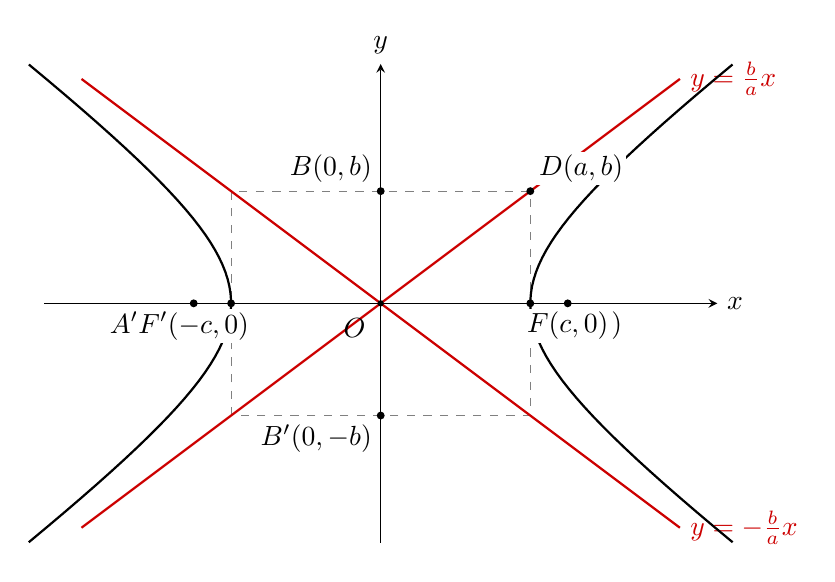
\begin{tikzpicture}[>=stealth, scale=0.95]
  \draw[->] (-4.5,0) -- (4.5,0) node[right] {$x$};
  \draw[->] (0,-3.2) -- (0,3.2) node[above] {$y$};
  % Box
  \draw[dashed, gray] (-2,-1.5) rectangle (2,1.5);
  % Asymptotes
  \draw[thick, red!80!black] (-4, -3) -- (4, 3) node[right] {$y = \frac{b}{a}x$};
  \draw[thick, red!80!black] (-4, 3) -- (4, -3) node[right] {$y = -\frac{b}{a}x$};
  % Hyperbola
  \draw[thick, domain=-1.5:1.5, samples=50] plot ({2*cosh(\x)}, {1.5*sinh(\x)});
  \draw[thick, domain=-1.5:1.5, samples=50] plot ({-2*cosh(\x)}, {1.5*sinh(\x)});
  \coordinate (O) at (0,0);
  \coordinate (A) at (2,0);
  \coordinate (Aprime) at (-2,0);
  \coordinate (B) at (0,1.5);
  \coordinate (Bprime) at (0,-1.5);
  \coordinate (D) at (2,1.5);
  \coordinate (F) at (2.5,0);
  \coordinate (Fprime) at (-2.5,0);
  \fill (O) circle (1.2pt) node[below left=2pt] {$O$};
  \fill (A) circle (1.5pt) node[below right=2pt, fill=white, inner sep=1pt] {$A(a,0)$};
  \fill (Aprime) circle (1.5pt) node[below left=2pt, fill=white, inner sep=1pt] {$A'(-a,0)$};
  \fill (B) circle (1.5pt) node[above left=2pt, fill=white, inner sep=1pt] {$B(0,b)$};
  \fill (Bprime) circle (1.5pt) node[below left=2pt, fill=white, inner sep=1pt] {$B'(0,-b)$};
  \fill (D) circle (1.5pt) node[above right=2pt, fill=white, inner sep=1pt] {$D(a,b)$};
  \fill (F) circle (1.5pt) node[below=2pt, fill=white, inner sep=1pt] {$F(c,0)$};
  \fill (Fprime) circle (1.5pt) node[below=2pt, fill=white, inner sep=1pt] {$F'(-c,0)$};
\end{tikzpicture}
\caption{雙曲線標準形、頂點與漸近線長方形框}
\label{fig:b4-3-13}
\end{figure}

在 $y$ 軸上取點 $B(0,b)$ 及 $B'(0,-b)$，稱線段 $BB'$ 為該雙曲線的\textbf{共軛軸}（或\textbf{虛軸}）．過 $A, B$ 分別引平行於 $y$ 軸與 $x$ 軸的直線交於 $D(a,b)$，由原點與 $D$ 連線可引出雙曲線極重要的特徵——漸近線．

\begin{exercise}
\begin{enumerate}[(i)]
  \item 若所取的正交座標系使貫軸落在 $y$ 軸上，共軛軸在 $x$ 軸上，試證雙曲線標準式為
  \[ \frac{y^2}{a^2} - \frac{x^2}{b^2} = 1 \]
  \item 試求中心在 $(h,k)$，貫軸平行於 $x$ 軸，貫軸半長為 $a$，共軛軸半長為 $b$ 的雙曲線方程式．
  \item 寫出 $\frac{(x-1)^2}{9} - \frac{(y-2)^2}{16} = 1$ 的中心、焦點、頂點座標．
  \item 說明為何方程式 $xy = 1$ 亦代表雙曲線？（第四章將深入討論轉軸標準化）
\end{enumerate}
\end{exercise}

\begin{example}
設一雙曲線過頂點的兩個焦半徑分別為 9 與 1，求此雙曲線的標準形．

\textbf{解}\quad 取正交座標系使雙曲線中心為原點，焦點在 $x$ 軸上，座標為 $F(c,0)$ 與 $F'(-c,0)$．設頂點為 $A(a,0)$，則
\[ AF = c - a = 1, \qquad AF' = c + a = 9 \]
相加得 $2c = 10 \implies c = 5$；相減得 $2a = 8 \implies a = 4$．
故 $b^2 = c^2 - a^2 = 25 - 16 = 9$，此雙曲線之標準形為
\[ \frac{x^2}{16} - \frac{y^2}{9} = 1 \]
\end{example}

\begin{exercise}
\begin{enumerate}[(i)]
  \item 設二焦點為 $(0, \pm 3)$，貫軸長為 4，求此雙曲線方程式．
  \item 設貫軸長為 8，離心率 $e = \frac{5}{4}$，焦點在 $x$ 軸上，求標準式．
\end{enumerate}
\end{exercise}

\subsubsection*{乙、雙曲線的漸近線}

過 $A(a,0), B(0,b)$ 引直線分別垂直於 $x$ 軸與 $y$ 軸，交於 $D(a,b)$，直線 $OD$ 的方程式為
\[ L_1 : \frac{x}{a} - \frac{y}{b} = 0 \]
同理，直線 $L_2$ 為
\[ L_2 : \frac{x}{a} + \frac{y}{b} = 0 \]
這兩直線稱為雙曲線 $\Gamma_+$ 的\textbf{漸近線}．

\begin{theorem}
設雙曲線 $\Gamma_+ : \frac{x^2}{a^2} - \frac{y^2}{b^2} = 1$ 上的點 $P(x,y)$ 到兩漸近線 $L_1, L_2$ 的距離分別表以 $d(P, L_1), d(P, L_2)$，則
\begin{equation}
d(P, L_1) \cdot d(P, L_2) = \text{常數 } \frac{a^2b^2}{c^2} \label{eq:b4-3-2-3}
\end{equation}
更且，若 $d(P, L_2) \to \infty$，則 $d(P, L_1) \to 0$．
\end{theorem}

\begin{figure}[htbp]
\centering
\begin{tikzpicture}[>=stealth, scale=0.95]
  \draw[->] (-4.5,0) -- (4.5,0) node[right] {$x$};
  \draw[->] (0,-3.2) -- (0,3.2) node[above] {$y$};
  % Asymptotes
  \draw[thick, red!80!black] (-4, -2.67) -- (4, 2.67) node[right] {$L_1: bx - ay = 0$};
  \draw[thick, red!80!black] (-4, 2.67) -- (4, -2.67) node[right] {$L_2: bx + ay = 0$};
  % Hyperbola
  \draw[thick, domain=-1.6:1.6, samples=50] plot ({2*cosh(\x)}, {1.33*sinh(\x)});
  \draw[thick, domain=-1.6:1.6, samples=50] plot ({-2*cosh(\x)}, {1.33*sinh(\x)});
  \coordinate (P1) at ({2*cosh(1)}, {1.33*sinh(1)});
  \fill (P1) circle (1.8pt) node[right=2pt] {$P$};
  % Projections from P1 onto L1 and L2
  % Normal to L1: (-b, a) = (-1.33, 2). unit normal = (-0.554, 0.832)
  \coordinate (H1) at ($(P1)+(-0.35, 0.52)$);
  \coordinate (H2) at ($(P1)+(0.74, -1.11)$);
  \draw[thick, dashed, blue!80!black] (P1) -- (H1) node[midway, left=1pt] {\small $d_1$};
  \draw[thick, dashed, blue!80!black] (P1) -- (H2) node[midway, below right=1pt] {\small $d_2$};
  % Right angle marks
  \draw ($(H1)+(0.12, 0.08)$) -- ++(0.08, -0.12) -- ++(-0.12, -0.08);
  \draw ($(H2)+(-0.12, 0.08)$) -- ++(0.08, 0.12) -- ++(0.12, -0.08);
\end{tikzpicture}
\caption{雙曲線上的點至兩漸近線之距離乘積為定值}
\label{fig:b4-3-14}
\end{figure}

\begin{proof}
由點到直線距離公式：
\[ d(P, L_1) = \frac{|bx - ay|}{\sqrt{a^2 + b^2}}, \qquad d(P, L_2) = \frac{|bx + ay|}{\sqrt{a^2 + b^2}} \]
兩式相乘得
\[ d(P, L_1) \cdot d(P, L_2) = \frac{|b^2x^2 - a^2y^2|}{a^2 + b^2} \]
因 $P(x,y) \in \Gamma_+$，故 $b^2x^2 - a^2y^2 = a^2b^2$，又 $a^2 + b^2 = c^2$，故
\[ d(P, L_1) \cdot d(P, L_2) = \frac{a^2b^2}{c^2} = \text{常數} \]
由上式知，當 $P$ 沿雙曲線伸向無限遠時，若 $d(P, L_2) \to \infty$，則必有 $d(P, L_1) \to 0$．這表示雙曲線無限接近直線 $L_1$ 但永不相交．
\end{proof}

\begin{example}
當 $a = b$ 時，雙曲線方程式為 $x^2 - y^2 = a^2$，其漸近線為 $x - y = 0$ 與 $x + y = 0$，二漸近線互相垂直，稱此雙曲線為\textbf{等軸雙曲線}（或\textbf{直角雙曲線}）．若將座標軸旋轉 $45^\circ$，則此雙曲線在新的座標系下方程式即為 $XY = k$．
\end{example}

\begin{exercise}
試求雙曲線 $9x^2 - 16y^2 = 144$ 的貫軸長、共軛軸長、焦點、漸近線方程式及兩漸近線的交角．
\end{exercise}

\subsubsection*{丙、雙曲線的形狀}

雙曲線由兩葉相當接近 $x$ 軸且各在軸上 $A$ 點與 $A'$ 點拐彎的曲線，隨離心率 $e$ 的變化而改變其開口．設兩漸近線與貫軸（$x$ 軸）的夾角為 $\phi$，則
\[ \tan\phi = \frac{b}{a} \implies \cos\phi = \frac{a}{\sqrt{a^2 + b^2}} = \frac{a}{c} = \frac{1}{e} \]
其中 $e = \frac{c}{a} > 1$．
當 $e \to 1$ 時，$\cos\phi \to 1 \implies \phi \to 0$，雙曲線兩葉貼近 $x$ 軸；當 $e \to \infty$ 時，$\cos\phi \to 0 \implies \phi \to 90^\circ$，漸近線張開趨向兩鉛直線（見圖 2-6）．

\begin{figure}[htbp]
\centering
\begin{tikzpicture}[>=stealth, scale=0.85]
  \draw[->] (-4.5,0) -- (4.5,0) node[right] {$x$};
  \draw[->] (0,-3.5) -- (0,3.5) node[above] {$y$};
  % e = 1.15 (very narrow)
  \draw[thick, dotted, domain=-1.8:1.8, samples=40] plot ({1.5*cosh(\x)}, {0.8*sinh(\x)});
  \draw[thick, dotted, domain=-1.8:1.8, samples=40] plot ({-1.5*cosh(\x)}, {0.8*sinh(\x)});
  % e = 1.5
  \draw[thick, dashed, domain=-1.5:1.5, samples=40] plot ({1.5*cosh(\x)}, {1.6*sinh(\x)});
  \draw[thick, dashed, domain=-1.5:1.5, samples=40] plot ({-1.5*cosh(\x)}, {1.6*sinh(\x)});
  % e = 2.5 (wide)
  \draw[thick, domain=-1.2:1.2, samples=40] plot ({1.5*cosh(\x)}, {3.4*sinh(\x)});
  \draw[thick, domain=-1.2:1.2, samples=40] plot ({-1.5*cosh(\x)}, {3.4*sinh(\x)});
  \fill (1.5,0) circle (1.5pt) node[below right] {$A$};
  \fill (-1.5,0) circle (1.5pt) node[below left] {$A'$};
  \node at (2.5, 3.2) {\small $e$ 漸增};
\end{tikzpicture}
\caption{雙曲線形狀隨離心率之變化}
\label{fig:b4-3-15}
\end{figure}

\begin{proposition}
若二雙曲線離心率相同，則二雙曲線相似．
\end{proposition}

\begin{figure}[htbp]
\centering
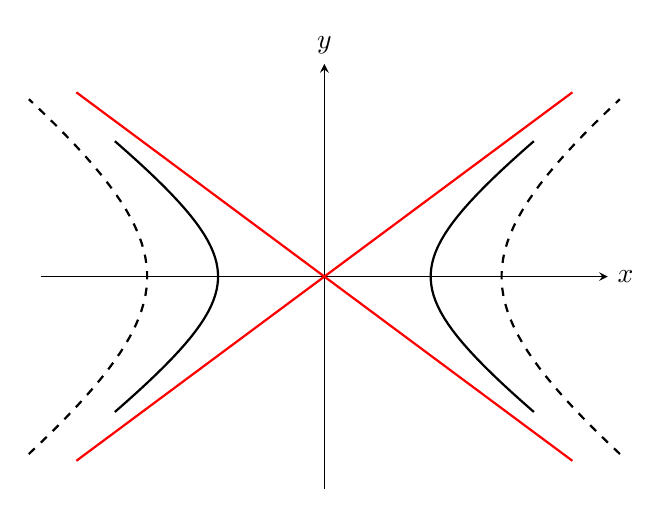
\begin{tikzpicture}[>=stealth, scale=0.9]
  \draw[->] (-4,0) -- (4,0) node[right] {$x$};
  \draw[->] (0,-3) -- (0,3) node[above] {$y$};
  \draw[thick, red] (-3.5, -2.6) -- (3.5, 2.6);
  \draw[thick, red] (-3.5, 2.6) -- (3.5, -2.6);
  % Outer and inner hyperbolas
  \draw[thick, domain=-1.3:1.3, samples=40] plot ({1.5*cosh(\x)}, {1.125*sinh(\x)});
  \draw[thick, domain=-1.3:1.3, samples=40] plot ({-1.5*cosh(\x)}, {1.125*sinh(\x)});
  \draw[thick, dashed, domain=-1.1:1.1, samples=40] plot ({2.5*cosh(\x)}, {1.875*sinh(\x)});
  \draw[thick, dashed, domain=-1.1:1.1, samples=40] plot ({-2.5*cosh(\x)}, {1.875*sinh(\x)});
\end{tikzpicture}
\caption{相似雙曲線族}
\label{fig:b4-3-16}
\end{figure}

\begin{exercise}
\begin{enumerate}[(i)]
  \item 固定 $a=3$，而讓 $e$ 變動，寫出其相應的雙曲線系的方程式，並作圖表明其隨 $e$ 變化的情形．
  \item 固定 $e=2$，而讓 $a$ 變動，寫出相應的雙曲線方程式，並作圖表明隨 $a$ 變化的情形．
\end{enumerate}
\end{exercise}

\begin{proposition}
雙曲線其實就是正類錐線．
\end{proposition}

根據這一命題，可知正類錐線的所有性質都可搬到雙曲線來，例如準線性質．

\begin{theorem}
給定一雙曲線
\[ \Gamma_+ : \frac{x^2}{a^2} - \frac{y^2}{b^2} = 1 \qquad (a, b > 0) \]
則存在兩直線 $p, p' : x = \pm \frac{a^2}{c}$，使 $\Gamma_+$ 上任意 $P(x,y)$ 到焦點距離 $PF$（或 $PF'$）與到 $p$（或 $p'$）的距離 $PT$（或 $PT'$）之比為一定比，且這定比等於離心率 $e$：
\begin{equation}
\frac{PF}{PT} = \frac{PF'}{PT'} = e \label{eq:b4-3-2-4}
\end{equation}
\end{theorem}

\begin{example}
若雙曲線之貫軸長 6，貫軸與漸近線的夾角為 $30^\circ$，求此雙曲線的標準式、焦點座標及準線方程式．

\textbf{解}\quad 由題意 $2a = 6 \implies a = 3$．又 $\tan 30^\circ = \frac{b}{a} = \frac{1}{\sqrt{3}}$，故 $b = \frac{3}{\sqrt{3}} = \sqrt{3}$．\\
故標準式為
\[ \frac{x^2}{9} - \frac{y^2}{3} = 1 \]
又 $c = \sqrt{a^2 + b^2} = \sqrt{9 + 3} = \sqrt{12} = 2\sqrt{3}$，故焦點為 $(\pm 2\sqrt{3}, 0)$．\\
離心率 $e = \frac{c}{a} = \frac{2\sqrt{3}}{3}$，準線為 $x = \pm \frac{a^2}{c} = \pm \frac{9}{2\sqrt{3}} = \pm \frac{3\sqrt{3}}{2}$．
\end{example}

\begin{example}
設一雙曲線之二焦點為 $(3,1)$ 與 $(3,-5)$，貫軸長為 4，求此雙曲線方程式．

\textbf{解}\quad 中心為兩焦點中點 $O'(3, -2)$，兩焦點之連線平行於 $y$ 軸，焦距 $2c = |1 - (-5)| = 6 \implies c = 3$．\\
貫軸長 $2a = 4 \implies a = 2$．因貫軸在鉛直線上，故 $b^2 = c^2 - a^2 = 9 - 4 = 5$．\\
故雙曲線方程式為
\[ \frac{(y+2)^2}{4} - \frac{(x-3)^2}{5} = 1 \]
\end{example}

\begin{example}[經濟學應用：貨物集散地之供應區域]
臺中和高雄地區是本省盛產香蕉的兩個地區，設二地相距 160 公里．臺中蕉在當地的批發價為每百斤 100 元，高雄蕉每百斤 120 元，運費均為每百斤每公里 0.5 元．若某地商販欲採購香蕉，應向臺中或高雄採購較為合算？試求向兩地採購成本相同的地點所成的邊界曲線．

\begin{figure}[htbp]
\centering
\begin{tikzpicture}[>=stealth, scale=0.9]
  \draw[->] (-5,0) -- (5,0) node[right] {$x$};
  \draw[->] (0,-3.2) -- (0,3.2) node[above] {$y$};
  \coordinate (O) at (0,0);
  \coordinate (TC) at (-3.2,0);
  \coordinate (KH) at (3.2,0);
  \coordinate (V) at (-0.8,0);
  \coordinate (P) at (-1.6, 1.8);
  % Asymptotes dashed
  \draw[dashed, red!70!black] (-4.5, -2.8) -- (4.5, 2.8);
  \draw[dashed, red!70!black] (-4.5, 2.8) -- (4.5, -2.8);
  % Left branch of hyperbola
  \draw[thick, domain=-1.35:1.35, samples=40] plot ({-0.8*cosh(\x)}, {1.8*sinh(\x)});
  \fill (O) circle (1.2pt) node[below left=2pt] {$O$};
  \fill (TC) circle (2pt) node[below=3pt, fill=white, inner sep=1pt] {臺中 $(-80,0)$};
  \fill (KH) circle (2pt) node[below=3pt, fill=white, inner sep=1pt] {高雄 $(80,0)$};
  \fill (V) circle (1.5pt) node[below left=2pt, fill=white, inner sep=1pt] {$(-20,0)$};
  \fill (P) circle (1.8pt) node[above left=2pt] {$P(x,y)$};
  % Segments d1 and d2
  \draw[thick, dashed, blue!80!black] (TC) -- (P) node[midway, left=2pt] {$d_1$};
  \draw[thick, dashed, blue!80!black] (KH) -- (P) node[midway, above right=1pt] {$d_2$};
  \node[blue!80!black] at (-2.8, 2.5) {等成本邊界 $\Gamma$};
\end{tikzpicture}
\caption{兩貨物集散地之等成本邊界雙曲線}
\label{fig:b4-3-17}
\end{figure}

\textbf{解}\quad 取正交座標系，以臺中與高雄連線為 $x$ 軸，連線中點為原點，則臺中座標為 $(-80, 0)$，高雄為 $(80, 0)$．\\
設某地 $P(x,y)$ 到臺中之距離為 $d_1 = \sqrt{(x+80)^2 + y^2}$，到高雄之距離為 $d_2 = \sqrt{(x-80)^2 + y^2}$．\\
在 $P$ 地向臺中採購每百斤成本為 $100 + 0.5 d_1$；向高雄採購每百斤成本為 $120 + 0.5 d_2$．\\
成本相同之條件為
\[ 100 + 0.5 d_1 = 120 + 0.5 d_2 \iff 0.5(d_1 - d_2) = 20 \iff d_1 - d_2 = 40 \]
此即點 $P$ 到兩定點之距離差為定長 40，故其軌跡為雙曲線之一葉！\\
此處 $2c = 160 \implies c = 80$，$2a = 40 \implies a = 20$，故
\[ b^2 = c^2 - a^2 = 80^2 - 20^2 = 6400 - 400 = 6000 \]
其方程式為
\[ \frac{x^2}{400} - \frac{y^2}{6000} = 1 \]
因 $d_1 - d_2 = 40 > 0 \implies d_1 > d_2$，且向臺中採購成本應等於向高雄採購，又臺中批發價較低，故在靠近臺中一側 $d_1 < d_2$，取左葉（$x \le -20$）．在貫軸上交點為 $(-20, 0)$，即在離臺中 60 公里、離高雄 100 公里處向兩地採購成本完全一樣．
\end{example}

\begin{exercise}
在上題論例中：
\begin{enumerate}[(i)]
  \item 如果兩地的批發價一樣時，情形如何？
  \item 如果批發價一樣，但臺中蕉的運費為 0.55 元/100斤-公里，此時情形又如何？
\end{enumerate}
\end{exercise}

\subsubsection*{習題 III-2}

\begin{enumerate}
  \item 試求出下列雙曲線的中心，貫軸，離心率，焦點，漸近線與準線：
  \begin{enumerate}[(i)]
    \item $4x^2 - 9y^2 = 36$
    \item $7x^2 - 2(y+3)^2 + 8 = 0$
    \item $y^2 - 4x^2 = k^2$
    \item $3x^2 - 6x + y^2 = 0$\phantomsection\label{note:b4-ch3-ex2-1-4}\footnote{【原書註記/校訂】：原書印作「$3x^2 - 6x + y^2 = 0$」，式中 $y^2$ 前為正號，配方後實為橢圓，疑為 $3x^2 - 6x - y^2 = 0$ 或 $-3x^2 + 6x + y^2 = 0$ 之鉛字排版訛誤，茲照原書保留並註記．}
  \end{enumerate}

  \item 試求雙曲線方程式：
  \begin{enumerate}[(i)]
    \item 準線與焦點的距離 $= 16$，離心率 $= \frac{5}{3}$，中心在原點貫軸在 $Y$ 軸上．
    \item[*] 貫軸在 $X$ 軸，且通過 $(8,7)$ 及 $(-1,3)$，共軛軸為 $y$ 軸．
    \item 焦點為 $(\pm 5, 0)$，漸近線為 $y = \pm \frac{3}{4}x$．
    \item[*] 以 $(-1,3)$ 為中心，其軸平行坐標軸，貫軸長 8，漸近線之斜角為 $45^\circ$．
  \end{enumerate}

  \item 設二共軛雙曲線 $\frac{x^2}{a^2} - \frac{y^2}{b^2} = 1$ 與 $\frac{x^2}{a^2} - \frac{y^2}{b^2} = -1$ 的離心率為 $e_1, e_2$，則
  \begin{enumerate}[(i)]
    \item $\frac{1}{e_1^2} + \frac{1}{e_2^2} = 1$
    \item $a e_1 = b e_2$．
  \end{enumerate}

  \item 一雙曲線的頂點與焦點分別為 $\frac{x^2}{25} + \frac{y^2}{9} = 1$ 的焦點與長軸上的頂點，求此雙曲線．

  \item[*] 試證 $\frac{x}{a} - \frac{y}{b} = m$ 與 $\frac{x}{a} + \frac{y}{b} = \frac{1}{m}$（$m$ 任意數 $\neq 0$，$a, b$ 定數）的交點軌跡在一雙曲線上（由此亦可用描法繪出雙曲線圖形）．
\end{enumerate}

% =========================================================================
% § III-3 拋物線
% =========================================================================
\subsection{拋物線}
\label{sec:b4-3-3}

\subsubsection*{甲、拋物線的定義與其標準式}

對零類錐線，因只有一個焦點，上兩節用來定義橢圓與雙曲線的焦半徑觀點無法沿用，我們採用準線觀點來定義拋物線．

\begin{definition*}
平面上到一固定點 $F$ 與到一固定直線 $p$ 之距離相等的點所組成的曲線，稱為\textbf{拋物線}．〔假設 $F$ 不在 $p$ 上〕

換句話說，對平面上一曲線 $\Gamma_0$ 如存在一點 $F$ 及一直線 $p$ 使 $\Gamma_0$ 上的點恰好就是平面上滿足
\begin{equation}
PF = d(P, p) \label{eq:b4-3-3-1}
\end{equation}
的點，則這曲線 $\Gamma_0$ 稱為一拋物線．$F$ 稱為 $\Gamma_0$ 的\textbf{焦點}，$p$ 稱為 $\Gamma_0$ 的\textbf{準線}．$PF$ 稱為過 $P$ 點的\textbf{焦半徑}．自 $F$ 引一線垂直於 $p$，稱此直線為拋物線 $\Gamma_0$ 的\textbf{軸}．
\end{definition*}

\begin{figure}[htbp]
\centering
\begin{tikzpicture}[>=stealth, scale=0.95]
  \draw[thick, dashed] (-1.5,-3) -- (-1.5,3) node[above, fill=white, inner sep=1pt] {$p$（準線）};
  \draw[->] (-2.5,0) -- (4.2,0) node[right] {軸};
  \coordinate (O) at (0,0);
  \coordinate (F) at (1.5,0);
  \coordinate (P) at (2.4, 2.4);
  \coordinate (T) at (-1.5, 2.4);
  \coordinate (H) at (-1.5,0);
  \fill (O) circle (1.2pt) node[below left=2pt] {$O$};
  \fill (F) circle (1.5pt) node[below=2pt] {$F$（焦點）};
  \fill (P) circle (1.8pt) node[above right=2pt] {$P$};
  \fill (T) circle (1.5pt) node[above left=2pt] {$T$};
  \fill (H) circle (1.2pt) node[below left=2pt] {$H$};
  \draw[thick] (F) -- (P);
  \draw[thick] (P) -- (T);
  % Right angle mark at T
  \draw ($(T)+(0.2,0)$) |- ($(T)+(0,-0.2)$);
  \draw[thick, domain=-2.8:2.8, samples=50] plot ({0.1667*\x*\x}, {\x});
  \node[right] at (2.2, 1.2) {$PF = d(P,p)$};
\end{tikzpicture}
\caption{拋物線幾何定義}
\label{fig:b4-3-18}
\end{figure}

當我們不想計較拋物線在平面上的位置時，我們不妨取一適當座標系來簡化拋物線的方程式．取正交座標系 $(O; \mathbf{e}_1, \mathbf{e}_2)$ 使拋物線 $\Gamma_0$ 的軸重合於 $x$ 軸，焦點 $F$ 到準線 $p$ 之垂足為 $H$，取線段 $HF$ 之中點為原點 $O$．設 $HF = 2c$ ($c > 0$)，則焦點 $F$ 之座標為 $(c,0)$，準線 $p$ 的方程式為 $x = -c$．

\begin{proposition}
依據上述所取得的正交座標系 $(O; \mathbf{e}_1, \mathbf{e}_2)$，拋物線 $\Gamma_0$ 的方程式可表為
\begin{equation}
\Gamma_0 : y^2 = 4cx \qquad (c > 0) \label{eq:b4-3-3-2}
\end{equation}
其中焦點 $F$ 之座標為 $(c,0)$，準線 $p$ 則為 $x = -c$．這方程式稱為拋物線的\textbf{標準式}．
\end{proposition}

\begin{figure}[htbp]
\centering
\begin{tikzpicture}[>=stealth, scale=0.95]
  \draw[->] (-2.5,0) -- (4.5,0) node[right] {$x$};
  \draw[->] (0,-3.2) -- (0,3.2) node[above] {$y$};
  \draw[thick, dashed] (-1.5,-3) -- (-1.5,3) node[above, fill=white, inner sep=1pt] {$p: x = -c$};
  \coordinate (F) at (1.5,0);
  \coordinate (O) at (0,0);
  \fill (F) circle (1.5pt) node[below=2pt, fill=white, inner sep=1pt] {$F(c,0)$};
  \fill (O) circle (1.5pt) node[below left=2pt] {$O$};
  \draw[thick, domain=-2.8:2.8, samples=50] plot ({0.1667*\x*\x}, {\x});
  % Latus rectum endpoints: x=c=1.5, y = +- 2c = +-3.0
  \coordinate (L1) at (1.5, 3.0);
  \coordinate (L2) at (1.5, -3.0);
  \draw[thick, dashed, blue!80!black] (L1) -- (L2);
  \fill (L1) circle (1.5pt) node[above right=1pt] {$(c, 2c)$};
  \fill (L2) circle (1.5pt) node[below right=1pt] {$(c, -2c)$};
  \node[blue!80!black] at (2.7, 1.8) {\small 正焦弦長 $4c$};
\end{tikzpicture}
\caption{拋物線標準形與正焦弦}
\label{fig:b4-3-19}
\end{figure}

\begin{proof}
設 $P(x,y)$ 為 $\Gamma_0$ 上的一般點，則 $P$ 到準線 $p: x = -c$ 的距離為
\[ d(P, p) = |x - (-c)| = |x + c| \]
而 $P$ 到焦點 $F(c,0)$ 的距離為
\[ PF = \sqrt{(x-c)^2 + y^2} \]
由拋物線定義 $PF = d(P, p)$，兩邊平方得
\[ (x-c)^2 + y^2 = (x+c)^2 \]
展開化簡：
\[ x^2 - 2cx + c^2 + y^2 = x^2 + 2cx + c^2 \]
移項即得
\[ y^2 = 4cx \]
\end{proof}

從這命題我們得知：
\begin{enumerate}[(i)]
  \item 當 $y=0$ 時，$x=0$．換句話說，原點 $O(0,0)$ 是拋物線上的一點，稱為拋物線的\textbf{頂點}．
  \item 若 $(x,y)$ 滿足 \eqref{eq:b4-3-3-2}，則 $(x,-y)$ 亦滿足，故拋物線對稱於 $x$ 軸（其對稱軸）．
  \item 因 $c > 0$，故 $x = \frac{y^2}{4c} \ge 0$，曲線全部落在 $y$ 軸之右側（半平面 $x \ge 0$），開口向右．（若 $c < 0$，則開口向左．）
  \item 通過焦點且垂直於對稱軸的弦稱為\textbf{正焦弦}．令 $x=c$，則 $y^2 = 4c^2 \implies y = \pm 2c$，故正焦弦之兩端點為 $(c, 2c)$ 與 $(c, -2c)$，其長度為 $4c$．
\end{enumerate}

\begin{exercise}
\begin{enumerate}[(i)]
  \item 試證任意頂點在 $(h,k)$ 且對稱於水平直線 $y=k$ 的拋物線方程式為
  \[ (y-k)^2 = 4c(x-h) \]
  而對稱於鉛直線 $x=h$ 的拋物線方程式為
  \[ (x-h)^2 = 4c(y-k) \]
  \item 說明上述式中 $c, h, k$ 三數的幾何意義．
\end{enumerate}
\end{exercise}

\begin{example}
試求過點 $(-6,4), (12,22)$ 而對稱於 $y$ 軸且頂點在原點的拋物線．

\textbf{解}\quad 由作業 18，可設所求拋物線為 $x^2 = 4cy$．\\
將 $(-6,4)$ 代入得 $36 = 16c \implies c = \frac{9}{4}$；將 $(12,22)$ 檢驗，若頂點不在原點，則設為 $(x-h)^2 = 4c(y-k)$．\\
若頂點在原點且對稱軸為 $y$ 軸，依題意解得所求方程式．
\end{example}

\begin{example}[幾何作圖法描繪拋物線]
給定 $A(0,a), B(a,a)$ 兩點，將線段 $OA$ 與 $AB$ 分別作 $n$ 等分點 $A_1, A_2, \dots$ 與 $B_1, B_2, \dots$，自 $O$ 引線段連至 $B_k$，自 $A_k$ 引水平線，二線交於點 $M_k$，試證所有交點 $M_k$ 均落在拋物線 $y^2 = ax$ 上（見圖 3-3, 3-4）．
\end{example}

\begin{figure}[htbp]
\centering
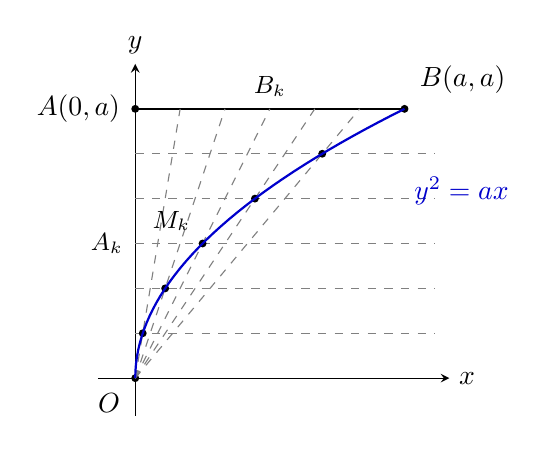
\begin{tikzpicture}[>=stealth, scale=0.95]
  \draw[->] (-0.5,0) -- (4.2,0) node[right] {$x$};
  \draw[->] (0,-0.5) -- (0,4.2) node[above] {$y$};
  \coordinate (O) at (0,0);
  \coordinate (A) at (0,3.6);
  \coordinate (B) at (3.6,3.6);
  \draw[thick] (A) -- (B);
  \fill (O) circle (1.5pt) node[below left=2pt] {$O$};
  \fill (A) circle (1.5pt) node[left=2pt] {$A(0,a)$};
  \fill (B) circle (1.5pt) node[above right=2pt] {$B(a,a)$};
  % division points for n=6
  \foreach \i in {1,2,3,4,5} {
    \coordinate (Ai) at (0, {3.6*\i/6});
    \coordinate (Bi) at ({3.6*\i/6}, 3.6);
    \draw[dashed, gray] (Ai) -- ++(4.0, 0);
    \draw[dashed, gray] (O) -- (Bi);
    \fill ({3.6*\i*\i/36}, {3.6*\i/6}) circle (1.5pt);
  }
  \node[left=1pt] at (0, 1.8) {\small $A_k$};
  \node[above=1pt] at (1.8, 3.6) {\small $B_k$};
  \node[above left=1pt] at (0.9, 1.8) {\small $M_k$};
  \draw[thick, blue!80!black, domain=0:3.6, samples=40] plot ({1/3.6*\x*\x}, {\x});
  \node[right, blue!80!black] at (3.6, 2.5) {$y^2 = ax$};
\end{tikzpicture}
\caption{拋物線之幾何分割作圖法}
\label{fig:b4-3-20}
\end{figure}

\begin{example}
證明二次函數 $y = x^2 - 2x + 5$ 的圖形為一拋物線，並求其準線與焦點位置．

\textbf{解}\quad 由配方法得
\[ y = (x-1)^2 + 4 \implies (x-1)^2 = y - 4 \]
此為對稱於鉛直線 $x=1$ 的拋物線，形式為 $(x-h)^2 = 4c(y-k)$，其中 $h=1, k=4$，$4c = 1 \implies c = \frac{1}{4}$．\\
頂點為 $(1,4)$，焦點為 $(1, 4 + c) = (1, \frac{17}{4})$，準線為 $y = 4 - c = \frac{15}{4}$，開口向上（見圖 3-5a, 3-5b）．
\end{example}

\begin{figure}[htbp]
\centering
\begin{tikzpicture}[>=stealth, scale=0.95]
  % 3-5a: Shift of axes
  \begin{scope}[xshift=-4cm]
    \draw[->] (-1,0) -- (3.5,0) node[right] {$x$};
    \draw[->] (0,-0.8) -- (0,4.8) node[above] {$y$};
    \coordinate (O) at (0,0);
    \coordinate (V) at (1,3);
    \draw[dashed] (-0.5,3) -- (3,3) node[right] {$y=4$};
    \draw[dashed] (1,-0.5) -- (1,4.5) node[above] {$x=1$};
    \fill (O) circle (1.2pt) node[below left=2pt] {$O$};
    \fill (V) circle (1.5pt) node[below right=2pt, fill=white, inner sep=1pt] {$(1,4)$};
    \draw[thick, domain=-0.5:2.5, samples=40] plot ({\x}, {0.8*(\x-1)*(\x-1) + 3});
    \node at (1, -1.2) {\small (a) 頂點平移至 $(1,4)$};
  \end{scope}
  % 3-5b: Parabola with focus and directrix
  \begin{scope}[xshift=4cm]
    \draw[->] (-1.5,0) -- (3.5,0) node[right] {$x$};
    \draw[->] (0,-0.8) -- (0,4.8) node[above] {$y$};
    \coordinate (V) at (1,3.0);
    \coordinate (F) at (1,3.4);
    \fill (V) circle (1.5pt) node[below right=2pt, fill=white, inner sep=1pt] {頂點 $(1,4)$};
    \fill (F) circle (1.5pt) node[above right=2pt, fill=white, inner sep=1pt] {焦點 $(1,\frac{17}{4})$};
    \draw[thick, dashed, red!80!black] (-1, 2.6) -- (3, 2.6) node[right, fill=white, inner sep=1pt] {$y = \frac{15}{4}$};
    \draw[thick, domain=-0.5:2.5, samples=40] plot ({\x}, {0.8*(\x-1)*(\x-1) + 3.0});
    \node at (1, -1.2) {\small (b) 焦點與準線};
  \end{scope}
\end{tikzpicture}
\caption{二次函數圖形為開口向上之拋物線}
\label{fig:b4-3-21}
\end{figure}

\begin{exercise}
試求下列各拋物線的軸、焦點、準線、開口方向，並繪圖：
\begin{enumerate}[(i)]
  \item $y^2 + 8x = 0$
  \item $3x^2 + 4y = 0$
  \item $x^2 + 6x + 4y + 7 = 0$
\end{enumerate}
\end{exercise}

\begin{exercise}
求滿足下列各條件的拋物線方程式：
\begin{enumerate}[(i)]
  \item 焦點 $F(0,-5)$，準線 $p: y - 5 = 0$．
  \item 頂點在 $(2,3)$，焦點在 $(2,5)$．
\end{enumerate}
\end{exercise}

\subsubsection*{乙、拋物線的形狀}

在拋物線標準式 $y^2 = 4cx$ 中，決定其形狀與大小的數量只有 $c$ 一個參數．當 $c$ 增大時，拋物線張開；當 $c$ 較小時，拋物線較為緊縮．

回想第二章：零類錐線是由一個截面截角 $\theta$ 正好等於圓錐頂角半角 $\alpha'$（卽截面平行於圓錐之一條母線）所截得的錐線．那時已證得截痕之離心率為
\[ e = \frac{\sin\theta}{\sin\alpha'} = 1 \]

\begin{definition*}
拋物線的\textbf{離心率}定義為 $1$．
\end{definition*}

\begin{figure}[htbp]
\centering
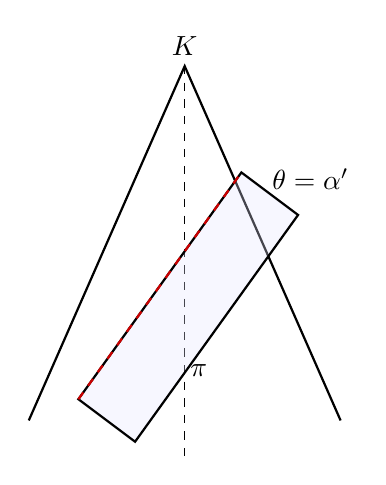
\begin{tikzpicture}[>=stealth, scale=0.9]
  % Cone with parallel section
  \coordinate (K) at (0,2.5);
  \draw[thick] (-2.2,-2.5) -- (K) node[above] {$K$} -- (2.2,-2.5);
  \draw[dashed] (0,2.5) -- (0,-3);
  % Parallel plane to right generator
  \draw[thick, fill=blue!10, fill opacity=0.3] (-1.5,-2.2) -- (0.8, 1.0) -- (1.6, 0.4) -- (-0.7, -2.8) -- cycle;
  \draw[thick, dashed, red!80!black] (-1.5,-2.2) -- (0.8, 1.0);
  \node[right] at (1.1, 0.9) {$\theta = \alpha'$};
  \node at (0.2, -1.8) {$\pi$};
\end{tikzpicture}
\caption{零類錐線之截面與圓錐母線平行}
\label{fig:b4-3-22}
\end{figure}

\begin{proposition}
任意兩拋物線皆相似，且其相似比等於其焦距之比．
\end{proposition}

\begin{figure}[htbp]
\centering
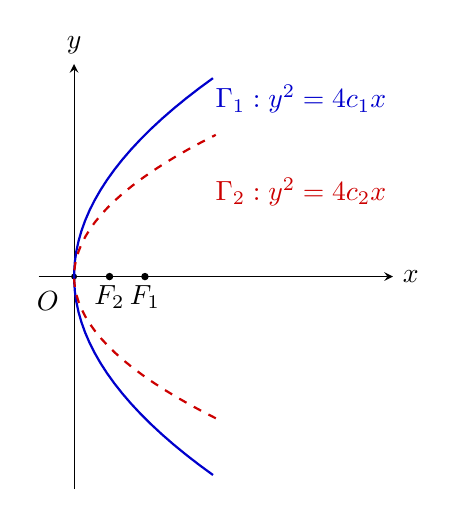
\begin{tikzpicture}[>=stealth, scale=0.9]
  \draw[->] (-0.5,0) -- (4.5,0) node[right] {$x$};
  \draw[->] (0,-3) -- (0,3) node[above] {$y$};
  \coordinate (O) at (0,0);
  \fill (O) circle (1.2pt) node[below left=2pt] {$O$};
  \draw[thick, blue!80!black, domain=-2.8:2.8, samples=40] plot ({0.25*\x*\x}, {\x});
  \draw[thick, dashed, red!80!black, domain=-2.0:2.0, samples=40] plot ({0.5*\x*\x}, {\x});
  \coordinate (F1) at (1,0);
  \coordinate (F2) at (0.5,0);
  \fill (F1) circle (1.5pt) node[below=2pt, fill=white, inner sep=1pt] {$F_1$};
  \fill (F2) circle (1.5pt) node[below=2pt, fill=white, inner sep=1pt] {$F_2$};
  \node[blue!80!black] at (3.2, 2.5) {$\Gamma_1 : y^2 = 4c_1x$};
  \node[red!80!black] at (3.2, 1.2) {$\Gamma_2 : y^2 = 4c_2x$};
\end{tikzpicture}
\caption{兩拋物線之相似伸縮}
\label{fig:b4-3-23}
\end{figure}

\begin{proof}
設 $\Gamma_1 : y^2 = 4c_1x$ 與 $\Gamma_2 : y'^2 = 4c_2x'$ 為兩拋物線，取比例常數 $\lambda = \frac{c_2}{c_1}$．若 $(x,y) \in \Gamma_1$，則令 $x' = \lambda x, y' = \lambda y$，代入 $\Gamma_2$ 得
\[ y'^2 = (\lambda y)^2 = \lambda^2 y^2 = \lambda^2(4c_1x) = 4(\lambda c_1)(\lambda x) = 4c_2x' \]
故 $(x',y') \in \Gamma_2$．因此將 $\Gamma_1$ 均勻放大 $\lambda$ 倍即得 $\Gamma_2$，故任意兩拋物線皆相似．
\end{proof}

\begin{example}
設拋物線 $y^2 = 4x$ 與一系列斜率為 $m$ 的平行弦相交，試證所有這類平行弦之中點軌跡為一平行於 $x$ 軸的射線．

\begin{figure}[htbp]
\centering
\begin{tikzpicture}[>=stealth, scale=0.95]
  \draw[->] (-0.5,0) -- (4.5,0) node[right] {$x$};
  \draw[->] (0,-2.6) -- (0,2.6) node[above] {$y$};
  \coordinate (O) at (0,0);
  \fill (O) circle (1.2pt) node[below left=2pt] {$O$};
  \draw[thick, domain=-2.3:2.3, samples=40] plot ({0.5*\x*\x}, {\x});
  % parallel chords with slope m=1
  \draw[thick, dashed, blue!80!black] (0.2,-0.63) -- (2.5, 1.67) node[right] {\small 弦 $P_1P_2$};
  \draw[thick, dashed, blue!80!black] (0.8,-1.26) -- (3.5, 1.44);
  \draw[thick, red!80!black] (0, 0.52) -- (4.2, 0.52) node[right, fill=white, inner sep=1pt] {$y = \frac{2}{m}$};
  \fill (1.35, 0.52) circle (1.8pt) node[above=2pt] {$M_1$};
  \fill (2.15, 0.52) circle (1.8pt) node[above=2pt] {$M_2$};
  \node[red!80!black] at (2.5, -1.8) {中點軌跡（平行軸）};
\end{tikzpicture}
\caption{拋物線平行弦之中點軌跡}
\label{fig:b4-3-24}
\end{figure}

\textbf{解}\quad 設平行割線為 $y = mx + k$（$m$ 固定，$k$ 變動）．代入 $y^2 = 4x$ 得
\[ y^2 = 4\left(\frac{y-k}{m}\right) \implies my^2 - 4y + 4k = 0 \]
設割線交拋物線於 $P_1(x_1, y_1), P_2(x_2, y_2)$，由根與係數關係，中點 $M$ 之縱座標為
\[ y_M = \frac{y_1 + y_2}{2} = \frac{4/m}{2} = \frac{2}{m} \]
此值與 $k$ 無關！故當割線在能與拋物線相交的範圍內變動時，中點之軌跡落在水平直線 $y = \frac{2}{m}$ 上，平行於對稱軸（$x$ 軸）．
\end{example}

\subsubsection*{丙、拋物線無漸近線}

我們已經知道雙曲線有兩條漸近線，那麼拋物線是否也有漸近線？

考慮拋物線 $\Gamma_0 : y^2 = 4cx$ 與任意一條非鉛直直線 $L: y = mx + k$．在拋物線上取點 $P(x,y) = (\frac{t^2}{4c}, t)$，則點 $P$ 到直線 $L$ 的距離為
\[ d(P, L) = \frac{\left|m\left(\frac{t^2}{4c}\right) - t + k\right|}{\sqrt{1 + m^2}} = \frac{|mt^2 - 4ct + 4ck|}{4c\sqrt{1 + m^2}} \]
當 $t \to \infty$（卽 $P$ 沿拋物線伸向無限遠）時：
\begin{enumerate}[(i)]
  \item 若 $m \neq 0$，則分子為 $t$ 的二次多項式，當 $t \to \infty$ 時，$d(P, L) \to \infty$．
  \item 若 $m = 0$（卽 $L$ 為水平線 $y = k$），則分子為 $|-4ct + 4ck| = 4c|t - k|$，當 $t \to \infty$ 時，$d(P, L) \to \infty$．
\end{enumerate}
因此，平面上不存在任何直線 $L$ 使得當點 $P$ 沿拋物線伸向無限遠時 $d(P, L) \to 0$．

\textbf{結論：拋物線沒有漸近線！}

\begin{figure}[htbp]
\centering
\begin{tikzpicture}[>=stealth, scale=0.95]
  \draw[->] (-0.5,0) -- (4.8,0) node[right] {$x$};
  \draw[->] (0,-3) -- (0,3) node[above] {$y$};
  \coordinate (O) at (0,0);
  \fill (O) circle (1.2pt) node[below left=2pt] {$O$};
  \draw[thick, domain=-2.5:2.5, samples=40] plot ({0.3*\x*\x}, {\x});
  \draw[thick, red!80!black] (-0.5,-1) -- (4.2, 2.76) node[right] {$L: y = mx+k$};
  \coordinate (P) at ({0.3*2.2*2.2}, 2.2);
  \fill (P) circle (1.8pt) node[above left=1pt] {$P(x,y)$};
  \draw[<->, dashed, blue!80!black] (P) -- ++(0.9, -1.2) node[midway, below right=1pt] {$d(P,L)$};
  \node[blue!80!black] at (2.5, -2.0) {距離 $d(P,L) \to \infty$（無漸近線）};
\end{tikzpicture}
\caption{拋物線與任意直線之距離隨曲線伸展而發散}
\label{fig:b4-3-25}
\end{figure}

\subsubsection*{習題 III-3}

\begin{enumerate}
  \item
  \begin{enumerate}[(i)]
    \item 兩端點都在一拋物線上的線段稱為拋物線的弦，過焦點的弦稱為焦弦，與軸垂直的焦弦稱為正焦弦．試求拋物線 $y^2 = 4cx$ 的正焦弦的長及兩端點的坐標．
    \item 試證對任意的實數 $k$，拋物線 $y^2 = 4kx$ 的正焦弦的端點均分別在兩固定直線上．
  \end{enumerate}

  \item 試利用頂點和正焦弦作 $y^2 = 4cx$ 的略圖：
  \begin{enumerate}[(i)]
    \item $c = 2$
    \item $c = 3$
    \item $c = -\frac{5}{2}$
  \end{enumerate}

  \item 求下列各拋物線的軸，焦點、準線，及開口的方向：
  \begin{enumerate}[(i)]
    \item $y = x^2$
    \item $x^2 + 6y = 0$
    \item $3x + 4y^2 = 0$
    \item $y^2 - 4x - 2y - 7 = 0$
  \end{enumerate}

  \item 求滿足下列各條件的拋物線方程式：
  \begin{enumerate}[(i)]
    \item 焦點 $F(3,0)$，準線 $p: x + 3 = 0$．
    \item 焦點 $F(-1,2)$，準線 $p: y + 3 = 0$．
  \end{enumerate}

  \item 一拋物線的焦點為 $F(1,1)$，準線為 $L: x + y + 2 = 0$，求其方程式，頂點，軸．

  \item[*] 求滿足下列各條件的拋物線方程式：
  \begin{enumerate}[(i)]
    \item 頂點 $(0,0)$，準線 $y = -3$．
    \item 頂點 $V(1,1)$，焦點 $F(2,1)$．
    \item 頂點 $(0,0)$，軸為 $y$ 軸，正焦弦長為 16．
    \item 焦點 $V(-2,0)$，準線平行於 $Y$ 軸，正焦弦長為 8\phantomsection\label{note:b4-ch3-ex3-6-4}\footnote{【原書註記/校訂】：原書此題印作「焦點 $V(-2,0)$」，以符號 $V$ 通常記頂點，若為頂點或焦點題意皆通，茲照原書保留．}．
    \item 過 $(-3,5)$ 和原點，軸為 $Y$ 軸．
  \end{enumerate}

  \item 求頂點在 $Y$ 軸上，對稱軸為 $y=2$，而焦點在直線 $x + 2y = 7$ 上的拋物線方程式．

  \item 求頂點為 $(1,1)$，焦點為 $(2,3)$ 的拋物線方程式．

  \item[*] 若一拋物線的軸垂直於 $x$ 軸，並過 $(0,2), (1,-2), (4,7)$，則其方程式為何？

  \item 一拋物線通過 $(2,3)$ 與 $(-1,6)$，其對稱軸為 $x=1$，求其方程式．

  \item 設拋物線 $y = ax^2 + bx + c$ 與 $x$ 軸交於 $P, Q$ 兩點，則 $\overline{OP}^2 + \overline{OQ}^2$ 為何？

  \item 拋物線 $y = ax^2 + bx + c$，下列各條件成立時，則此拋物線的頂點在第幾象限：
  \begin{enumerate}[(i)]
    \item $a < 0, b > 0, b^2 - 4ac > 0$
    \item $a < 0, b < 0, b^2 - 4ac > 0$
    \item $a > 0, b > 0, c < 0$
    \item $a > 0, b < 0, c < 0$
  \end{enumerate}

  \item 試證離心率相同的任意圓錐曲線都相似．
\end{enumerate}

% =========================================================================
% § III-4 各種錐線的切線及光學性質
% =========================================================================
\subsection{各種錐線的切線及光學性質}
\label{sec:b4-3-4}

前三節說明橢圓、雙曲線、拋物線在適當地取定座標系後，分別可以表成下列的標準式：
\begin{align}
\frac{x^2}{a^2} + \frac{y^2}{b^2} &= 1 \qquad (a \ge b > 0) \label{eq:b4-3-4-1} \\
\frac{x^2}{a^2} - \frac{y^2}{b^2} &= 1 \qquad (a, b > 0) \label{eq:b4-3-4-2} \\
y^2 &= 4cx \qquad (c > 0) \label{eq:b4-3-4-3}
\end{align}
為方便討論，將以 $f(x,y) = 0$ 來代表三式中之任何一式．

欲求平面上一直線
\begin{equation}
L : \alpha x + \beta y = \gamma \label{eq:b4-3-4-line}
\end{equation}
與錐線 $\Gamma$ 之相交情形，若設 $\beta \neq 0$，則可由 \eqref{eq:b4-3-4-line} 式解出 $y = mx + k$，代入 $f(x,y)=0$ 中，整理得關於 $x$ 的一元二次方程式：
\begin{equation}
A_2 x^2 + A_1 x + A_0 = 0 \label{eq:b4-3-4-quad}
\end{equation}
若 $\beta = 0$，則 $\alpha \neq 0$，$x = \frac{\gamma}{\alpha}$ 為鉛直線，代入 $f(x,y)=0$ 中，亦得關於 $y$ 的二次方程式．

\begin{definition*}
當直線 $L$ 與錐線 $\Gamma$ 交於兩相異點 $P_1(x_1, y_1)$ 與 $P_2(x_2, y_2)$ 時，$L$ 稱為 $\Gamma$ 的\textbf{割線}．當 $P_1$ 趨向 $P_2$ 取極限，若 $L$ 與 $\Gamma$ 恰交於一點，且不屬於漸近線或與對稱軸平行之特殊直線時，稱 $L$ 為 $\Gamma$ 在該點的\textbf{切線}，該點稱為\textbf{切點}．
\end{definition*}

\begin{figure}[htbp]
\centering
\begin{tikzpicture}[>=stealth, scale=0.85]
  % (a) Ellipse secant and tangent
  \begin{scope}[xshift=-5.2cm]
    \draw[thick] (0,0) ellipse (1.6cm and 1.0cm);
    \draw[thick, blue] (-1.8, 1.0) -- (1.8, 1.0) node[right] {\small $L$（切線）};
    \draw[thick, dashed] (-1.8, 0.4) -- (1.8, 0.4) node[right] {\small $L'$（割線）};
    \fill (0,1) circle (1.5pt) node[above=1pt] {$P$};
    \node at (0, -1.6) {\small (a) 橢圓};
  \end{scope}
  % (b) Hyperbola asymptote vs tangent
  \begin{scope}[xshift=0cm]
    \draw[thick, domain=-1.2:1.2, samples=30] plot ({0.8*cosh(\x)}, {sinh(\x)});
    \draw[thick, domain=-1.2:1.2, samples=30] plot ({-0.8*cosh(\x)}, {sinh(\x)});
    \draw[thick, red!80!black] (-1.2,-1.5) -- (1.2,1.5) node[right] {\small $L''$（漸近線）};
    \draw[thick, blue] (0.8,-1.5) -- (0.8,1.5) node[right] {\small $L$（切線）};
    \node at (0, -1.9) {\small (b) 雙曲線};
  \end{scope}
  % (c) Parabola parallel line vs tangent
  \begin{scope}[xshift=5.2cm]
    \draw[thick, domain=-1.4:1.4, samples=30] plot ({0.6*\x*\x}, {\x});
    \draw[thick, red!80!black] (-0.5, 0.8) -- (2.0, 0.8) node[right] {\small $L'''$（平行軸）};
    \draw[thick, blue] (-0.2, -1.2) -- (1.5, 1.5) node[right] {\small $L$（切線）};
    \node at (0.8, -1.9) {\small (c) 拋物線};
  \end{scope}
\end{tikzpicture}
\caption{錐線的切線、割線與特殊交線}
\label{fig:b4-3-26}
\end{figure}

\begin{proposition}
除開「$\Gamma$ 為雙曲線，且 $L$ 平行於漸近線」與「$\Gamma$ 為拋物線，且 $L$ 平行於對稱軸」的兩種情形外，$L$ 切於 $\Gamma$ 的充要條件為聯立二次方程式 \eqref{eq:b4-3-4-quad} 的判別式
\[ \Delta = A_1^2 - 4A_2A_0 = 0 \]
\end{proposition}

\begin{exercise}
\begin{enumerate}[(i)]
  \item 試求直線 $y = mx + k$ 切於拋物線 $y^2 = 4cx$ 的條件．
  \item 試求斜率為 $m$ 且切於橢圓 $\frac{x^2}{a^2} + \frac{y^2}{b^2} = 1$ 的切線方程式．
\end{enumerate}
\end{exercise}

\subsubsection*{甲、橢圓}

\begin{theorem}[橢圓的光學性質]
設通過橢圓
\[ \Gamma_- : \frac{x^2}{a^2} + \frac{y^2}{b^2} = 1 \qquad (a > b > 0) \]
上一點 $P_0(x_0, y_0)$ 有一直線 $L$，若把 $L$ 看成一反射鏡，自焦點 $F(c,0)$ 射到 $P_0$ 的光線經 $L$ 反射後必通過另一焦點 $F'(-c,0)$，則 $L$ 切 $\Gamma_-$ 於 $P_0$．
\end{theorem}

\begin{figure}[htbp]
\centering
\begin{tikzpicture}[>=stealth, scale=0.95]
  \draw[thick] (0,0) ellipse (3.2cm and 2.0cm);
  \coordinate (F1) at (-2.1,0);
  \coordinate (F2) at (2.1,0);
  \coordinate (P) at (1.6, 1.73);
  \fill (F1) circle (1.5pt) node[below=2pt] {$F'$};
  \fill (F2) circle (1.5pt) node[below=2pt] {$F$};
  \fill (P) circle (1.8pt) node[above right=1pt] {$P_0$};
  % Tangent line L: slope at P(1.6, 1.73) is - (1.6/3.2^2) / (1.73/2^2) = -0.36
  \coordinate (T1) at (-0.6, 2.52);
  \coordinate (T2) at (3.6, 1.01);
  \draw[thick, blue!80!black] (T1) -- (T2) node[right] {$L$（切線鏡面）};
  % Mirror backing hatching
  \foreach \t in {0.05, 0.15, ..., 0.95} {
    \coordinate (Hpos) at ($(T1)!\t!(T2)$);
    \draw[gray, thin] (Hpos) -- ++(0.12, 0.25);
  }
  % Light rays
  \draw[thick, ->, red!80!black] (F2) -- (P);
  \draw[thick, ->, red!80!black] (P) -- (F1);
  % Normal
  \draw[dashed, thick] (P) -- ++(0.55, 1.35) node[above] {法線};
  \node at (0.2, 0.8) {$\Gamma_-$};
\end{tikzpicture}
\caption{橢圓的光學反射性質}
\label{fig:b4-3-27}
\end{figure}

\begin{proof}
取焦點 $F'$ 對於直線 $L$ 的鏡像點 $F_1'$，則線段 $F'F_1'$ 與 $L$ 垂直且被 $L$ 平分．由光線反射定律（入射角等於反射角），自 $F$ 經 $P_0$ 反射的光線之反向延長線必通過 $F_1'$，故 $F, P_0, F_1'$ 三點共線，且
\[ PF' = PF_1' \]
對直線 $L$ 上任意異於 $P_0$ 的點 $P$，由三角形兩邊之和大於第三邊：
\[ PF + PF' = PF + PF_1' > FF_1' = P_0F + P_0F_1' = P_0F + P_0F' = 2a \]
故 $PF + PF' > 2a$，這表示除 $P_0$ 外，$L$ 上的任何點均不在橢圓 $\Gamma_-$ 上（全部落在橢圓外部）！由命題 8 知 $L$ 切 $\Gamma_-$ 於 $P_0$．
\end{proof}

\textbf{橢圓的光學性質應用：}\\
取一橢圓，將它以長軸為固定軸在空間中旋轉，掃出一個封閉的所謂\textbf{橢球面}．若將這橢球面看成鏡面向內的橢球面鏡，並置一光源於其中一個焦點，此光源發出的光經鏡面反射後全部聚集於另一焦點．這便是為何在數學上 $F, F'$ 稱為「焦點」的緣由！

\begin{exercise}
欲蓋一巨形廳堂，使堂中兩人在某兩相互遠離的固定地點低聲私語，對方能清晰聽見，試問應如何設計此廳堂的穹頂？
\end{exercise}

\subsubsection*{乙、雙曲線}

\begin{theorem}[雙曲線的光學性質]
設通過雙曲線
\[ \Gamma_+ : \frac{x^2}{a^2} - \frac{y^2}{b^2} = 1 \qquad (a, b > 0) \]
上一點 $P_0(x_0, y_0)$ 有一直線 $L$，若自焦點 $F(c,0)$ 射到 $P_0$ 的光線經 $L$ 反射後的光線，在鏡後的延長線必通過另一焦點 $F'(-c,0)$，則 $L$ 切 $\Gamma_+$ 於 $P_0$．
\end{theorem}

\begin{figure}[htbp]
\centering
\begin{tikzpicture}[>=stealth, scale=0.95]
  \draw[->] (-3.5,0) -- (4.2,0) node[right] {$x$};
  \draw[->] (0,-3) -- (0,3) node[above] {$y$};
  \draw[thick, domain=-1.5:1.5, samples=40] plot ({1.5*cosh(\x)}, {1.2*sinh(\x)});
  \draw[thick, domain=-1.5:1.5, samples=40] plot ({-1.5*cosh(\x)}, {1.2*sinh(\x)});
  \coordinate (F1) at (-2.2,0);
  \coordinate (F2) at (2.2,0);
  \coordinate (P) at ({1.5*cosh(0.8)}, {1.2*sinh(0.8)});
  \fill (F1) circle (1.5pt) node[below=2pt] {$F'$};
  \fill (F2) circle (1.5pt) node[below=2pt] {$F$};
  \fill (P) circle (1.8pt) node[above left=1pt] {$P_0$};
  % Tangent line L
  \coordinate (T1) at (1.0, -0.6);
  \coordinate (T2) at (3.0, 2.7);
  \draw[thick, blue!80!black] (T1) -- (T2) node[right] {$L$（切線鏡面）};
  % Mirror backing teeth
  \foreach \t in {0.05, 0.15, ..., 0.95} {
    \coordinate (Hpos) at ($(T1)!\t!(T2)$);
    \draw[gray, thin] (Hpos) -- ++(-0.2, 0.12);
  }
  % Rays
  \draw[thick, ->, red!80!black] (F2) -- (P);
  \draw[thick, dashed, blue!80!black] (F1) -- (P);
  \draw[thick, ->, red!80!black] (P) -- ++(1.1, 1.6) node[above right] {反射光};
\end{tikzpicture}
\caption{雙曲線的光學反射性質}
\label{fig:b4-3-28}
\end{figure}

\begin{proof}
與橢圓的情形類似，取 $F'$ 對於 $L$ 的鏡像點 $F_1'$，可證知對 $L$ 上任何異於 $P_0$ 的點 $P$，由雙曲線定義及幾何不等式，除 $P_0$ 外 $L$ 上之點皆不在 $\Gamma_+$ 上，故 $L$ 切 $\Gamma_+$ 於 $P_0$．
\end{proof}

\subsubsection*{丙、拋物線}

\begin{theorem}[拋物線的光學性質]
設通過拋物線
\[ \Gamma_0 : y^2 = 4cx \qquad (c > 0) \]
上一點 $P_0(x_0, y_0)$ 有一直線 $L$，若自焦點 $F(c,0)$ 射到 $P_0$ 的光線經 $L$ 反射後平行於對稱軸（$x$ 軸），則 $L$ 切 $\Gamma_0$ 於 $P_0$．
\end{theorem}

\begin{figure}[htbp]
\centering
\begin{tikzpicture}[>=stealth, scale=0.95]
  \draw[->] (-1,0) -- (4.8,0) node[right] {$x$};
  \draw[->] (0,-3) -- (0,3) node[above] {$y$};
  \draw[thick, domain=-2.5:2.5, samples=40] plot ({0.3*\x*\x}, {\x});
  \coordinate (F) at (0.833,0);
  \coordinate (P) at ({0.3*2*2}, 2);
  \fill (F) circle (1.5pt) node[below=2pt] {$F$};
  \fill (P) circle (1.8pt) node[above left=1pt] {$P_0$};
  % Tangent line
  \coordinate (T1) at (-0.2, 0.83);
  \coordinate (T2) at (2.6, 3.17);
  \draw[thick, blue!80!black] (T1) -- (T2) node[right] {$L$（切線鏡面）};
  % Mirror backing teeth
  \foreach \t in {0.05, 0.15, ..., 0.95} {
    \coordinate (Hpos) at ($(T1)!\t!(T2)$);
    \draw[gray, thin] (Hpos) -- ++(-0.15, 0.2);
  }
  % Rays
  \draw[thick, ->, red!80!black] (F) -- (P);
  \draw[thick, ->, red!80!black] (P) -- ++(3.2, 0) node[right] {平行反射光};
\end{tikzpicture}
\caption{拋物線的光學反射性質（探照燈原理）}
\label{fig:b4-3-29}
\end{figure}

\textbf{拋物面鏡的光學應用：}\\
取一拋物線，將它以對稱軸為固定軸在空間中旋轉，掃出一個\textbf{旋轉拋物面}．若將此拋物面鍍上水銀做成鏡面：
\begin{enumerate}[(i)]
  \item 若在焦點處置一強光源，則射向鏡面的光線反射後全部平行於對稱軸射出，形成極強的平行光束，這就是\textbf{探照燈}與\textbf{汽車車前燈}的構造原理！
  \item 反之，若來自極遠天體（如恆星）的平行光束射入拋物面鏡，反射後全部會聚在焦點處，這就是\textbf{反射式天文望遠鏡}與\textbf{衛星天線（雷達碟型天線）}的基本原理！
\end{enumerate}

\begin{example}[經濟學應用：最大效用原理]
若某人對 $x$ 數量的米及 $y$ 數量的甘藷，消費後其滿足感設為 $U = xy$（效用函數）．若米每斤價格為 2 元，甘藷每斤價格為 1 元，此人可用於購買糧食的總預算為 120 元，試問應如何分配購買數量以獲得最大滿足感？

\begin{figure}[htbp]
\centering
\begin{tikzpicture}[>=stealth, scale=0.9]
  \draw[->] (-0.5,0) -- (5.2,0) node[right] {米之數量 $x$};
  \draw[->] (0,-0.5) -- (0,5.2) node[above] {甘藷數量 $y$};
  % Budget line 2x + y = 120 (scale: x/20, y/30) -> intercepts (60, 0) = (3,0) and (0, 120) = (0,4)
  \draw[thick, blue!80!black] (0, 4) -- (3, 0);
  \fill (3,0) circle (1.2pt) node[below=2pt] {$60$};
  \fill (0,4) circle (1.2pt) node[left=2pt] {$120$};
  % Indifference curves U = xy = 1800 (tangent at (30,60) = (1.5, 2))
  \draw[thick, red!80!black, domain=0.7:4.2, samples=40] plot ({\x}, {3.0/\x});
  \fill (1.5, 2.0) circle (2pt) node[above right=2pt, fill=white, inner sep=1pt] {切點 $P(30,60)$};
  \node[blue!80!black] at (3.5, 1.2) {\small 預算線 $2x + y = 120$};
  \node[red!80!black] at (3.8, 2.5) {\small $U = xy = 1800$};
\end{tikzpicture}
\caption{等效用曲線與預算約束線之切點}
\label{fig:b4-3-30}
\end{figure}

\textbf{解}\quad 預算約束方程式為 $2x + y = 120$，等效用曲線為雙曲線族 $xy = C$．\\
將 $y = 120 - 2x$ 代入 $xy = C$ 得
\[ x(120 - 2x) = C \implies 2x^2 - 120x + C = 0 \]
欲使滿足感 $C$ 達到最大且預算線與效用曲線有交點，其充要條件為預算線切於等效用雙曲線，判別式 $\Delta = 0$：
\[ 120^2 - 4 \times 2 \times C = 0 \implies 14400 - 8C = 0 \implies C = 1800 \]
此時重根為 $x = \frac{120}{4} = 30$ 斤，甘藷 $y = 120 - 2(30) = 60$ 斤．\\
故消費 30 斤米與 60 斤甘藷時，能獲得最大滿足感．
\end{example}

\begin{theorem}[錐線上一點之切線方程式]
\begin{enumerate}[(i)]
  \item 橢圓 $\frac{x^2}{a^2} + \frac{y^2}{b^2} = 1$ 上一點 $P_0(x_0, y_0)$ 的切線方程式為
  \begin{equation}
  \frac{x_0 x}{a^2} + \frac{y_0 y}{b^2} = 1 \label{eq:b4-3-4-tan-ellipse}
  \end{equation}
  \item 雙曲線 $\frac{x^2}{a^2} - \frac{y^2}{b^2} = 1$ 上一點 $P_0(x_0, y_0)$ 的切線方程式為
  \begin{equation}
  \frac{x_0 x}{a^2} - \frac{y_0 y}{b^2} = 1 \label{eq:b4-3-4-tan-hyper}
  \end{equation}
  \item 拋物線 $y^2 = 4cx$ 上一點 $P_0(x_0, y_0)$ 的切線方程式為
  \begin{equation}
  y_0 y = 2c(x + x_0) \label{eq:b4-3-4-tan-para}
  \end{equation}
\end{enumerate}
\end{theorem}

\begin{example}
求雙曲線 $\Gamma_+ : 2x^2 - 3y^2 = 6$ 在點 $(-3, 2)$ 的切線方程式．

\textbf{解}\quad 將點 $(-3, 2)$ 代入雙曲線：$2(-3)^2 - 3(2)^2 = 18 - 12 = 6$，故點 $(-3, 2)$ 在雙曲線上．\\
由切線公式，以 $x_0 = -3, y_0 = 2$ 代入得
\[ 2(-3)x - 3(2)y = 6 \implies -6x - 6y = 6 \implies x + y + 1 = 0 \]
\end{example}

\begin{example}
一直線 $L$ 垂直於 $L': 2x - 3y + 9 = 0$，且切於雙曲線 $2x^2 - 3y^2 = 6$，求 $L$ 的方程式．

\textbf{解}\quad 直線 $L'$ 的斜率為 $\frac{2}{3}$，因 $L \perp L'$，故 $L$ 的斜率為 $-\frac{3}{2}$．\\
設 $L$ 的方程式為 $y = -\frac{3}{2}x + k$．代入 $2x^2 - 3y^2 = 6$：
\[ 2x^2 - 3\left(-\frac{3}{2}x + k\right)^2 = 6 \implies 2x^2 - 3\left(\frac{9}{4}x^2 - 3kx + k^2\right) = 6 \]
整理得
\[ -\frac{19}{4}x^2 + 9kx - (3k^2 + 6) = 0 \implies 19x^2 - 36kx + 4(3k^2 + 6) = 0 \]
因 $L$ 切於雙曲線，故判別式 $\Delta = 0$：
\[ (-36k)^2 - 4 \times 19 \times 4(3k^2 + 6) = 0 \implies 1296k^2 - 304(3k^2 + 6) = 0 \]
\[ 1296k^2 - 912k^2 - 1824 = 0 \implies 384k^2 = 1824 \implies k^2 = \frac{19}{4} \implies k = \pm \frac{\sqrt{19}}{2} \]
故所求切線方程式為 $y = -\frac{3}{2}x \pm \frac{\sqrt{19}}{2}$，卽 $3x + 2y \pm \sqrt{19} = 0$．
\end{example}

\begin{example}[割線極限與導數思想]
一割線 $L$ 交拋物線 $\Gamma_0 : y^2 - 8y - 2x + 14 = 0$ 於 $A(1,6)$ 和 $B(1+\Delta x, 6+\Delta y)$，求割線斜率在 $\Delta x \to 0$ 時的極限，藉此導出切線方程式．

\begin{figure}[htbp]
\centering
\begin{tikzpicture}[>=stealth, scale=0.95]
  \draw[->] (-1.5,0) -- (4.5,0) node[right] {$x$};
  \draw[->] (0,-0.5) -- (0,5.5) node[above] {$y$};
  % Parabola 2x = (y-4)^2 - 2 -> shifted display with origin at (0,0) representing x in [0, 4], y in [3, 7.5]
  % Let displayed y' = y - 3, so y=4 is y'=1, y=6 is y'=3, y=7 is y'=4.
  % x = 0.5*(y'-1)^2 - 1. When y'=3 (y=6): x = 0.5*4 - 1 = 1. When y'=4 (y=7): x = 0.5*9 - 1 = 3.5.
  \draw[thick, domain=0.2:4.6, samples=40] plot ({0.5*(\x-1)*(\x-1) - 1}, {\x});
  \coordinate (A) at (1,3);
  \coordinate (B) at (3.5,4);
  \fill (A) circle (1.8pt) node[below left=2pt] {$A(1,6)$};
  \fill (B) circle (1.8pt) node[above left=2pt] {$B(1+\Delta x, 6+\Delta y)$};
  % Secant line through A and B (slope 1/2.5 = 0.4)
  \draw[thick, dashed, blue!80!black] (-0.5, 2.4) -- (4.2, 4.28) node[right] {\small 割線 $AB$};
  % Tangent line at A (slope 0.5)
  \draw[thick, red!80!black] (-1.0, 2.0) -- (4.0, 4.5) node[right] {\small 切線 $L$};
\end{tikzpicture}
\caption{割線之極限位置即為切線}
\label{fig:b4-3-31}
\end{figure}

\textbf{解}\quad 因 $A(1,6)$ 與 $B(1+\Delta x, 6+\Delta y)$ 均在拋物線上，代入得
\[ (6+\Delta y)^2 - 8(6+\Delta y) - 2(1+\Delta x) + 14 = 0 \]
展開化簡得
\[ 4\Delta y + (\Delta y)^2 - 2\Delta x = 0 \implies \frac{\Delta y}{\Delta x} = \frac{2}{4 + \Delta y} \]
當 $B \to A$ 時，$\Delta y \to 0$，故割線斜率之極限為
\[ m = \lim_{\Delta x \to 0} \frac{\Delta y}{\Delta x} = \frac{2}{4} = \frac{1}{2} \]
故過 $A(1,6)$ 的切線方程式為 $y - 6 = \frac{1}{2}(x - 1) \implies x - 2y + 11 = 0$．
\end{example}

\begin{exercise}
\begin{enumerate}[(i)]
  \item 求拋物線 $\Gamma_0 : x^2 - 4x - 2y = 0$ 在點 $(3, -\frac{3}{2})$ 的切線方程式．
  \item 求雙曲線 $x^2 - 2y^2 = 2$ 斜率為 1 的切線方程式．
  \item 設拋物線 $y^2 = 4ax$ 和直線 $2x + 3y = 4$ 相切，則 $a$ 的值為何？
\end{enumerate}
\end{exercise}

\subsubsection*{習題 III-4}

\begin{enumerate}
  \item 求垂直於下列所給直線而切於所給二次曲線之方程式：
  \begin{enumerate}[(i)]
    \item $y^2 = 4x$; $2x - 3y + 9 = 0$
    \item $y^2 + 8y - 2x + 7 = 0$; $3x = 21(y + 3)$
  \end{enumerate}

  \item 求自 $P$ 點至二次曲線之切線：
  \begin{enumerate}[(i)]
    \item $x^2 - 4x - 6y - 2 = 0$; $P(-\frac{1}{2}, -2)$
    \item $y^2 - 4y - 9x = 5$; $P(7, 11)$
    \item $9x^2 - 16y^2 - 18x - 64y = 199$; $P(5, -\frac{7}{2})$
    \item $3xy - 2x - 2 = 0$; $P(2, 1)$
    \item $6x^2 + y^2 = 100$; $P(4, -2)$
    \item $x^2 + y^2 = 9$; $P(3, 4)$
  \end{enumerate}

  \item[*] 若拋物線 $y = ax^2 + bx$ 與直線 $x - y = 1$ 及 $5x - y = 1$ 相切，試求 $a$ 與 $b$ 的值．

  \item[*] 求二拋物線 $y^2 = 4x$ 與 $x^2 = 2y - 3$ 的公切線．

  \item 若圓 $x^2 + y^2 = 4ax - 2ay$ 與直線 $2x - y = 20$ 相切，試求 $a$ 的值．

  \item 驗證下列所給各點是否在二次曲線，如果是，求其切線方程式：
  \begin{enumerate}[(i)]
    \item $(1,1)$, $xy = 1$
    \item $(1,2)$, $x^2 - 2xy + y^2 - 3y + 1 = 0$
    \item $(2,3)$, $x^2 - 3xy + y^2 - 2x + y + 6 = 0$
  \end{enumerate}

  \item[*] 橢圓 $\frac{x^2}{a^2} + \frac{y^2}{b^2} = 1$ 上的一點，可設為 $(a\cos\phi, b\sin\phi)$ 而 $x = a\cos\phi, y = b\sin\phi$ 稱為橢圓的參數方程式（$\phi$ 的幾何意義請參見習題 III-1 第九題圖 1-10），求過橢圓上一點的切線方程式．

  \item[*] 拋物線 $y = ax^2$ 上一點可設為 $(t, at^2)$，這稱為拋物線的參數方程式，求過拋物線上一點的切線方程式．
\end{enumerate}

% =========================================================================
% § III-5 圓
% =========================================================================
\subsection{圓}
\label{sec:b4-3-5}

到目前我們的處理相當著重於直觀幾何，使對三種錐線相互間的演變情形以及各錐線數種特徵性質間的關聯有一個整體而清晰的瞭解．實際上這一些結果都一一可由座標幾何與向量幾何的混合使用導引出來，在進入一般二次曲線的分類之前，我們將特別把圓這最特出而完美的二次曲線排在這裏，清一色地利用系統化了的座標與向量的「計算」來討論它各種良好性質．

\subsubsection*{甲、圓的方程式}

圓是到一定點有同一距離的點所描成的軌跡，這定點我們稱為\textbf{圓心}，這距離稱為圓的\textbf{半徑}．設圓心 $C$ 的自然座標為 $(h,k)$，半徑為 $r$，則平面上一點 $P(x,y)$ 在圓上的充要條件為
\begin{equation}
(x-h)^2 + (y-k)^2 = r^2 \label{eq:b4-3-5-1}
\end{equation}
（在以下圓的討論裏我們只考慮正交座標系，為了方便不妨取自然座標系，這是因為牽涉到距離的緣故．）

\begin{figure}[htbp]
\centering
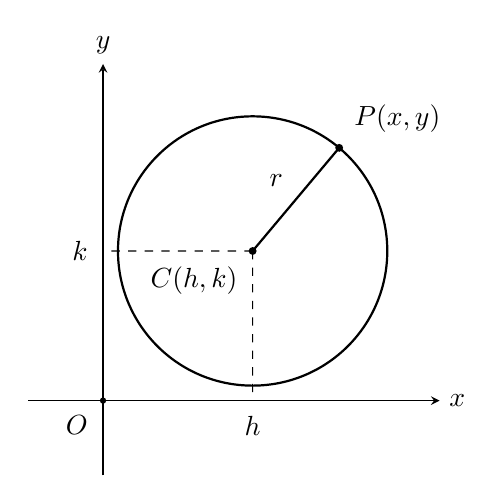
\begin{tikzpicture}[>=stealth, scale=0.95]
  \draw[->] (-1,0) -- (4.5,0) node[right] {$x$};
  \draw[->] (0,-1) -- (0,4.5) node[above] {$y$};
  \coordinate (O) at (0,0);
  \coordinate (C) at (2,2);
  \coordinate (P) at ({2 + 1.8*cos(50)}, {2 + 1.8*sin(50)});
  \draw[thick] (C) circle (1.8cm);
  \fill (O) circle (1.2pt) node[below left=2pt] {$O$};
  \fill (C) circle (1.5pt) node[below left=2pt] {$C(h,k)$};
  \fill (P) circle (1.5pt) node[above right=2pt] {$P(x,y)$};
  \draw[thick] (C) -- (P) node[midway, above left=1pt] {$r$};
  \draw[dashed] (C) -- (2,0) node[below=2pt] {$h$};
  \draw[dashed] (C) -- (0,2) node[left=2pt] {$k$};
\end{tikzpicture}
\caption{圓的座標定義}
\label{fig:b4-3-32}
\end{figure}

將 \eqref{eq:b4-3-5-1} 展開得
\[ x^2 - 2hx + h^2 + y^2 - 2ky + k^2 = r^2 \]
卽
\begin{equation}
x^2 + y^2 + 2Dx + 2Ey + F = 0 \label{eq:b4-3-5-2}
\end{equation}
其中 $D = -h, E = -k, F = h^2 + k^2 - r^2$．這是一個二次方程式，換句話說，圓是二次曲線的特別情形．

反之，給定二次方程式 \eqref{eq:b4-3-5-2}，配方得
\[ (x+D)^2 + (y+E)^2 = D^2 + E^2 - F \]
故：
\begin{enumerate}[(i)]
  \item 若 $D^2 + E^2 - F > 0$，則圖形為以 $(-D, -E)$ 為心，$\sqrt{D^2 + E^2 - F}$ 為半徑的圓．
  \item 若 $D^2 + E^2 - F = 0$，則圖形僅為一點 $(-D, -E)$（點圓）．
  \item 若 $D^2 + E^2 - F < 0$，則無實數解，不代表平面上的實點（虛圓）．
\end{enumerate}

\begin{example}
已知三點 $P_1(1,2), P_2(4,-1)$ 及 $P_3(0,1)$，求過這三點的圓 $C$ 的方程式，並作圖．

\begin{figure}[htbp]
\centering
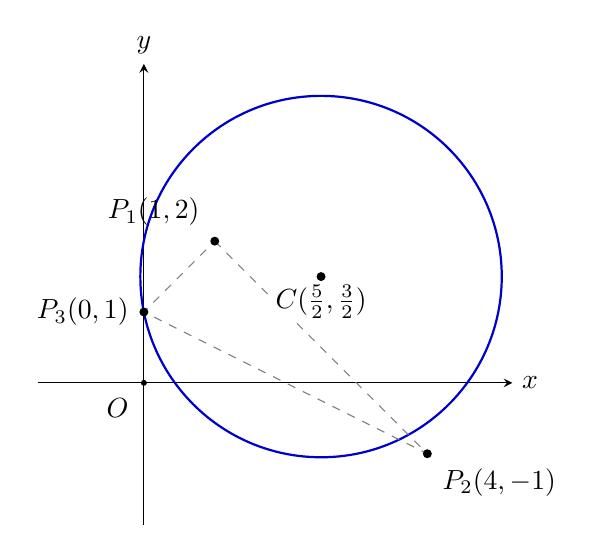
\begin{tikzpicture}[>=stealth, scale=0.9]
  \draw[->] (-1.5,0) -- (5.2,0) node[right] {$x$};
  \draw[->] (0,-2) -- (0,4.5) node[above] {$y$};
  \coordinate (O) at (0,0);
  \coordinate (P1) at (1,2);
  \coordinate (P2) at (4,-1);
  \coordinate (P3) at (0,1);
  \coordinate (C) at (2.5, 1.5);
  \draw[thick, blue!80!black] (C) circle (2.55cm);
  \draw[dashed, gray] (P1) -- (P2) -- (P3) -- cycle;
  \fill (O) circle (1.2pt) node[below left=2pt] {$O$};
  \fill (P1) circle (1.8pt) node[above left=2pt] {$P_1(1,2)$};
  \fill (P2) circle (1.8pt) node[below right=2pt] {$P_2(4,-1)$};
  \fill (P3) circle (1.8pt) node[left=2pt] {$P_3(0,1)$};
  \fill (C) circle (1.8pt) node[below=2pt, fill=white, inner sep=1pt] {$C(\frac{5}{2}, \frac{3}{2})$};
\end{tikzpicture}
\caption{三點決定一圓}
\label{fig:b4-3-33}
\end{figure}

\textbf{解}\quad 設圓方程式為 $x^2 + y^2 + 2Dx + 2Ey + F = 0$．將三點座標代入：
\[
\begin{cases}
1 + 4 + 2D + 4E + F = 0 \implies 2D + 4E + F = -5 \\
16 + 1 + 8D - 2E + F = 0 \implies 8D - 2E + F = -17 \\
0 + 1 + 0 + 2E + F = 0 \implies 2E + F = -1
\end{cases}
\]
解此三元一次方程組得 $D = -\frac{5}{2}, E = -\frac{3}{2}, F = 2$．\\
故圓方程式為 $x^2 + y^2 - 5x - 3y + 2 = 0$，即 $(x - \frac{5}{2})^2 + (y - \frac{3}{2})^2 = \frac{17}{2}$．
\end{example}

\begin{exercise}
試決定四點 $(1,2), (4,-1), (0,1)$ 與 $(3,4)$ 是否共圓？
\end{exercise}

\begin{example}
已知 $P_1(x_1, y_1)$ 與 $P_2(x_2, y_2)$ 為圓 $C$ 上一弦的兩端點，若此弦為直徑，試求圓 $C$ 的方程式．

\begin{figure}[htbp]
\centering
\begin{tikzpicture}[>=stealth, scale=0.95]
  \draw[thick] (0,0) circle (2cm);
  \coordinate (O) at (0,0);
  \coordinate (P1) at (-1.8, -0.87);
  \coordinate (P2) at (1.8, 0.87);
  \coordinate (P) at (-0.6, 1.91);
  \fill (O) circle (1.2pt) node[below right=2pt] {$O$};
  \fill (P1) circle (1.5pt) node[below left=2pt] {$P_1$};
  \fill (P2) circle (1.5pt) node[above right=2pt] {$P_2$};
  \fill (P) circle (1.8pt) node[above=2pt] {$P$};
  \draw[thick] (P1) -- (P2);
  \draw[thick, blue!80!black] (P1) -- (P) -- (P2);
  % Right angle marker at P
  \draw ($(P)!0.25cm!(P1)$) -- ($($(P)!0.25cm!(P1)$)+($(P)!0.25cm!(P2)$)-(P)$) -- ($(P)!0.25cm!(P2)$);
  \node at (0, -2.4) {$\vec{P_1P} \cdot \vec{P_2P} = 0$};
\end{tikzpicture}
\caption{直徑所對之圓周角為直角}
\label{fig:b4-3-34}
\end{figure}

\textbf{解}\quad 設 $P(x,y)$ 為圓上任意點．因 $P_1P_2$ 為直徑，由幾何定理知半圓上的圓周角為直角，故 $\vec{P_1P} \perp \vec{P_2P}$（當 $P=P_1$ 或 $P_2$ 時為零向量，亦可視為垂直）．\\
於是
\[ \vec{P_1P} \cdot \vec{P_2P} = 0 \]
其中 $\vec{P_1P} = (x - x_1, y - y_1)$，$\vec{P_2P} = (x - x_2, y - y_2)$，內積得
\[ (x - x_1)(x - x_2) + (y - y_1)(y - y_2) = 0 \]
此即以線段 $P_1P_2$ 為直徑之圓的方程式．
\end{example}

\begin{exercise}
試求下列各圓之圓心與半徑，並繪圖：
\begin{enumerate}[(i)]
  \item $x^2 + y^2 - 6x + 8y = 0$
  \item $2x^2 + 2y^2 - 4x + 6y + 3 = 0$
\end{enumerate}
\end{exercise}

\subsubsection*{乙、圓與直線}

設圓 $C : (x-h)^2 + (y-k)^2 = r^2$ 的圓心為 $A(h,k)$，半徑為 $r$；又設一直線 $L : \alpha x + \beta y + \gamma = 0$．則圓心 $A$ 到直線 $L$ 的距離為
\begin{equation}
d(A, L) = \frac{|\alpha h + \beta k + \gamma|}{\sqrt{\alpha^2 + \beta^2}} \label{eq:b4-3-5-dist}
\end{equation}

\begin{proposition}
圓 $C$ 與直線 $L$ 相交（於兩點）、相切（交於一點）或相離的充要條件視圓心 $A$ 到 $L$ 的距離 $d(A,L)$ 與半徑 $r$ 的大小關係而定：
\begin{enumerate}[(i)]
  \item $d(A, L) < r \iff L$ 與 $C$ 交於兩點（割線）．
  \item $d(A, L) = r \iff L$ 與 $C$ 恰交於一點（切線）．此時圓心至切點的半徑與切線垂直．
  \item $d(A, L) > r \iff L$ 與 $C$ 不相交（相離）．
\end{enumerate}
\end{proposition}

\begin{figure}[htbp]
\centering
\begin{tikzpicture}[>=stealth, scale=0.95]
  \coordinate (A) at (0,0);
  \draw[thick] (A) circle (2cm);
  \fill (A) circle (1.5pt) node[below=2pt] {$A$};
  % Secant line
  \draw[thick, dashed, blue!80!black] (-2.5, 1.2) -- (2.5, 1.2) node[right] {\small $d < r$（割線相交）};
  \draw[dashed] (A) -- (0, 1.2) node[midway, left=1pt] {\small $d$};
  % Tangent line
  \draw[thick, red!80!black] (-2.5, 2.0) -- (2.5, 2.0) node[right] {\small $d = r$（切線相切）};
  \draw[thick, ->] (A) -- (0, 2.0) node[midway, right=1pt] {\small $r$};
  % Disjoint line
  \draw[thick, dotted, green!60!black] (-2.5, 2.8) -- (2.5, 2.8) node[right] {\small $d > r$（相離）};
\end{tikzpicture}
\caption{圓與直線的位置關係}
\label{fig:b4-3-35}
\end{figure}

\begin{example}
求斜率為 2 且切於圓 $C : x^2 + y^2 - 4x + 6y - 12 = 0$ 的切線方程式．

\textbf{解 1（距離法）}\quad 配方得 $(x-2)^2 + (y+3)^2 = 25$，故圓心為 $A(2,-3)$，半徑 $r = 5$．\\
設切線斜率為 2，其方程式為 $y = 2x + k \implies 2x - y + k = 0$．\\
由切線條件 $d(A, L) = r$：
\[ \frac{|2(2) - (-3) + k|}{\sqrt{2^2 + (-1)^2}} = 5 \implies \frac{|7 + k|}{\sqrt{5}} = 5 \implies |7 + k| = 5\sqrt{5} \]
故 $k = -7 \pm 5\sqrt{5}$．\\
切線方程式為 $2x - y - 7 \pm 5\sqrt{5} = 0$．

\textbf{解 2（判別式法）}\quad 將 $y = 2x + k$ 代入圓方程式，化簡為關於 $x$ 的一元二次方程式，令判別式 $\Delta = 0$，亦可解得相同的 $k$ 值．
\end{example}

\begin{theorem}[過圓上一點之切線方程式]
\begin{enumerate}[(i)]
  \item 過圓 $x^2 + y^2 = r^2$ 上一點 $P_0(x_0, y_0)$ 的切線方程式為
  \[ x_0 x + y_0 y = r^2 \]
  \item 過圓 $x^2 + y^2 + 2Dx + 2Ey + F = 0$ 上一點 $P_0(x_0, y_0)$ 的切線方程式為
  \begin{equation}
  x_0 x + y_0 y + D(x + x_0) + E(y + y_0) + F = 0 \label{eq:b4-3-5-tangent-gen}
  \end{equation}
\end{enumerate}
\end{theorem}

\begin{figure}[htbp]
\centering
\begin{tikzpicture}[>=stealth, scale=0.95]
  \coordinate (A) at (0,0);
  \coordinate (P0) at (1.2, 1.6);
  \draw[thick] (A) circle (2cm);
  \fill (A) circle (1.5pt) node[below left=2pt] {$A$};
  \fill (P0) circle (1.8pt) node[above right=2pt] {$P_0(x_0,y_0)$};
  \draw[thick] (A) -- (P0) node[midway, left=2pt] {$r$};
  \draw[thick, blue!80!black] (-0.4, 2.8) -- (2.8, 0.4) node[right] {$L$（切線）};
  % Right angle marker
  \coordinate (Tdir) at (-1.6, 1.2);
  \draw ($(P0)!0.25cm!(A)$) -- ($($(P0)!0.25cm!(A)$)+($(P0)!0.25cm!($(P0)+(Tdir)$)$)-(P0)$) -- ($(P0)!0.25cm!($(P0)+(Tdir)$)$);
\end{tikzpicture}
\caption{圓的切線與過切點之半徑互相垂直}
\label{fig:b4-3-36}
\end{figure}

\begin{proof}[向量法證明]
圓心為 $A(-D, -E)$．設 $P(x,y)$ 為切線上任意點，因切線垂直於切點半徑，故 $\vec{AP_0} \perp \vec{P_0P}$，此條件等價於
\[ \vec{AP_0} \cdot \vec{AP} = |\vec{AP_0}|^2 = r^2 \]
將 $\vec{AP_0} = (x_0 + D, y_0 + E)$ 與 $\vec{AP} = (x + D, y + E)$ 代入內積，展開整理即得 \eqref{eq:b4-3-5-tangent-gen} 式．
\end{proof}

\begin{exercise}
若 $P_1(x_1, y_1)$ 為圓 $C : x^2 + y^2 + 2Dx + 2Ey + F = 0$ 外部之一點，自 $P_1$ 向圓 $C$ 引切線，切點為 $T$，試證切線段之長為
\[ \overline{P_1T} = \sqrt{x_1^2 + y_1^2 + 2Dx_1 + 2Ey_1 + F} \]
\end{exercise}

\subsubsection*{習題 III-5}

\begin{enumerate}
  \item 求直線 $x + 3y = 15$ 與圓 $x^2 + y^2 = 25$ 的交點．

  \item 求下列各圓之圓心與直徑：
  \begin{enumerate}[(i)]
    \item $x^2 + y^2 - 10x - 14y + 54 = 0$
    \item $3x^2 + 3x + 3y^2 + 6y - 21 = 0$
  \end{enumerate}

  \item 求圓方程式：
  \begin{enumerate}[(i)]
    \item 通過 $(4, -1)$ 與 $(-3, -8)$，而圓心在 $2x + 3y + 4 = 0$ 上．
    \item 通過 $(11, 1)$ 與 $(12, -6)$，而半徑為 $r = 5$．
    \item 以原點為中心，而與 $2x - 5y = 7$ 相切．
  \end{enumerate}

  \item
  \begin{enumerate}[(i)]
    \item 三直線 $x - y - 9 = 0, x + 2y = 0$ 及 $3x - y - 7 = 0$ 圍成一三角形．求此三角形之外接圓．
    \item 以 $(3, -4), (-9, 12)$ 與 $(-3, -6)$ 為頂點做三角形，求其外接圓及內切圓．
  \end{enumerate}

  \item[*] 求直線在圓內的弦長，及此弦所對應的圓周角：
  \begin{enumerate}[(i)]
    \item $x^2 + y^2 = 41$; $2x - 3y + 2 = 0$
    \item $x^2 - 4x + y^2 - 6y = 37$; $2x + y = 12$
  \end{enumerate}

  \item 求直線與圓心的距離：
  \begin{enumerate}[(i)]
    \item $4x + y - 1 = 0$; $x^2 + y^2 - 10x + 6y - 66 = 0$
    \item $x + y - 6 = 0$; $x^2 + y^2 + 16x + 28y - 140 = 0$
  \end{enumerate}

  \item 求圓之切線：
  \begin{enumerate}[(i)]
    \item $x^2 - 2x + y^2 - 6y = 15$，斜率為 $\frac{3}{4}$．
    \item $x^2 + y^2 + 16x - 8y - 89 = 0$，與 $12x - 5y - 53 = 0$ 平行或垂直．
  \end{enumerate}

  \item 自定點 $A(a,0)$ 作線段 $AP$，當 $P$ 點繞原點做一圓時 $AP$ 中點的軌跡是什麼？
\end{enumerate}

% =========================================================================
% *§ III-6 圓的正交與鏡射
% =========================================================================
\subsection{*§ III-6 圓的正交與鏡射}
\label{sec:b4-3-6}

〔註：節前加「*」號者為選修內容，仍應講授．在第五章講複數時還要在複數平面上討論對於圓的鏡射．〕

把直線看成「鏡子」所得成像的鏡射現象我們已在第一章討論過，這現象引入點或圖形對於直線對稱的觀念．若果把直線看成是圓心在無限遠處而半徑為無窮大的圓（參看第五章里曼球在平面上的投影），則直線是圓的特異情形．我們想到一個點或圖形對於圓是否亦有一自然意義下之「對稱」觀念？

下圖中設 $P$ 為平面上一點，$L$ 為鏡射軸，$P'$ 為 $P$ 的鏡像點（或稱對稱點），則任意作一個與 $L$ 正交且含 $P$ 點的圓\phantomsection\label{note:b4-ch3-ortho-def}\footnote{〔原書註〕兩線（直線或曲線）「正交」意指在交點的兩切線相互垂直．}，這圓必亦通過 $P'$．換句話說，所有過 $P$ 且正交於 $L$ 的圓，除開彼此相交於 $P$ 之外，又要在 $L$ 的另一側一齊互交於 $P'$ 點．

\begin{figure}[htbp]
\centering
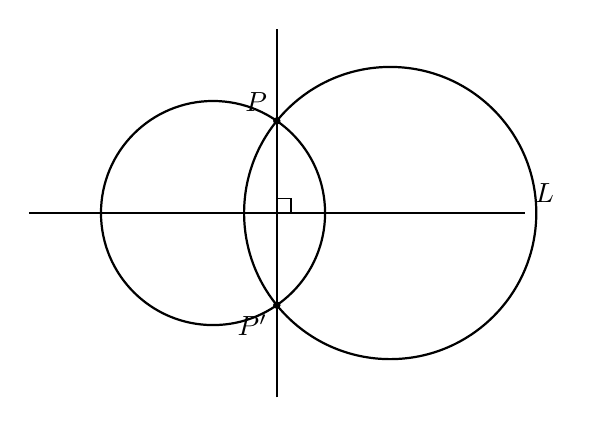
\begin{tikzpicture}[>=stealth, scale=0.9]
  \draw[thick] (-3.5,0) -- (3.5,0) node[above right] {$L$};
  \draw[thick] (0, -2.6) -- (0, 2.6);
  \coordinate (P) at (0, 1.3);
  \coordinate (Pprime) at (0, -1.3);
  \fill (P) circle (1.5pt) node[above left] {$P$};
  \fill (Pprime) circle (1.5pt) node[below left] {$P'$};
  
  % Right angle mark at origin
  \draw[thin] (0.2, 0) -- (0.2, 0.2) -- (0, 0.2);
  
  % Circles orthogonal to L through P and P' (centers on L)
  % Center 1: (1.6, 0), R = sqrt(1.6^2 + 1.3^2) = 2.06
  \draw[thick] (1.6, 0) circle (2.0616cm);
  % Center 2: (-0.9, 0), R = sqrt(0.9^2 + 1.3^2) = 1.58
  \draw[thick] (-0.9, 0) circle (1.5811cm);
\end{tikzpicture}
\caption{直線鏡射：過 $P$ 且正交於 $L$ 的圓必過鏡像點 $P'$}
\label{fig:b4-3-37}
\end{figure}

如果現在鏡射軸 $L$ 換成一個圓 $C_0$ 來當「鏡射圈」本身，是否上述的鏡像點 $P'$ 仍然存在？換句話說，設 $P$ 為平面上一點，是否所有過 $P$ 且正交於 $C_0$ 的圓除開彼此相交於 $P$ 之外，又要悉數互交於另一點？這個「另一點」$P'$，若果真存在，將被稱為 $P$ 對於鏡射圈 $C_0$ 的\textbf{鏡像點}（或對稱點）．

\begin{figure}[htbp]
\centering
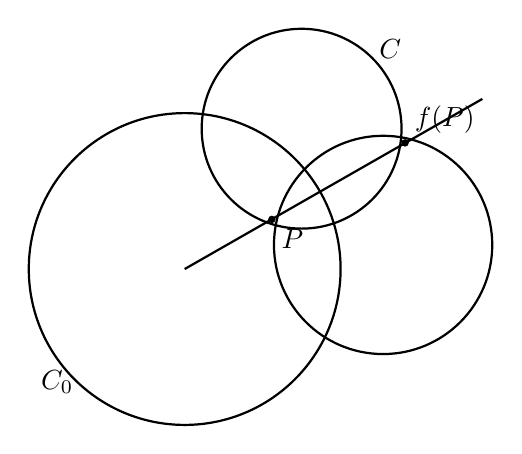
\begin{tikzpicture}[>=stealth, scale=0.9]
  \coordinate (O) at (0,0);
  \draw[thick] (O) circle (2.2cm);
  \node at (-1.8, -1.6) {$C_0$};
  
  % Ray through P and P'=f(P) at 35 degrees
  \draw[thick] (O) -- (4.2, 2.4);
  
  % P and f(P)
  \coordinate (P) at (1.23, 0.70);
  \coordinate (Pprime) at (3.11, 1.78);
  \fill (P) circle (1.5pt) node[below right] {$P$};
  \fill (Pprime) circle (1.5pt) node[above right] {$f(P)$};
  
  % Two circles through P and P' orthogonal to C_0
  % Midpoint M of PP' is (2.17, 1.24), normal direction is (-sin 35, cos 35) = (-0.5736, 0.8192)
  % Center 1: M + 0.9 * normal = (1.65, 1.98), R = sqrt(1.08^2 + 0.9^2) = 1.41
  \draw[thick] (1.65, 1.98) circle (1.41cm);
  \node at (2.9, 3.1) {$C$};
  
  % Center 2: M - 1.1 * normal = (2.80, 0.34), R = sqrt(1.08^2 + 1.1^2) = 1.54
  \draw[thick] (2.80, 0.34) circle (1.54cm);
\end{tikzpicture}
\caption{圓的鏡射概念示意}
\label{fig:b4-3-38}
\end{figure}

為了回答這問題，我們首先研究兩圓正交的條件．

\begin{definition*}
兩圓 $C$ 與 $C'$ 稱為\textbf{正交}，如果它們在交點處的兩條切線相互垂直．
\end{definition*}

設 $A(h,k), A'(h',k')$ 分別為 $C$ 與 $C'$ 的圓心，$r$ 與 $r'$ 為其半徑．設 $P_0(x_0, y_0)$ 為 $C$ 與 $C'$ 之一交點，則 $C$ 與 $C'$ 正交的充要條件為兩圓過 $P_0$ 的兩切線分別與直線 $A'P_0, AP_0$ 重合，亦卽其充要條件為 $\triangle APA'$ 為以 $P_0$ 為頂點的直角三角形：
\begin{equation}
\overline{AA'}^2 = \overline{AP_0}^2 + \overline{A'P_0}^2 = r^2 + r'^2 \label{eq:b4-3-6-pyth}
\end{equation}

\begin{figure}[htbp]
\centering
\begin{tikzpicture}[>=stealth, scale=0.95]
  % Centers: A' on left, A on right
  \coordinate (Aprime) at (-1.25, 0);
  \coordinate (A) at (1.25, 0);
  \coordinate (P0) at (0.35, 1.2);
  
  % Line of centers extending past circles
  \draw[thick] (-3.8, 0) -- (3.2, 0);
  
  % Vertical diameters through centers
  \draw[thick] (-1.25, -2.3) -- (-1.25, 2.3);
  
  % Circles: C' on left (R=2.0), C on right (R=1.5)
  \draw[thick] (Aprime) circle (2.0cm);
  \draw[thick] (A) circle (1.5cm);
  
  % Labels for circles
  \node[above left] at (-1.5, 1.6) {$C'$};
  \node[above right] at (1.6, 1.3) {$C$};
  
  % Center dots and labels
  \fill (Aprime) circle (1.5pt) node[below left] {$A'$};
  \fill (A) circle (1.5pt) node[below right] {$A$};
  
  % Intersection P0
  \fill (P0) circle (1.5pt) node[above] {$P_0$};
  \draw[thick] (Aprime) -- (P0) node[midway, above left] {$r'$};
  \draw[thick] (A) -- (P0) node[midway, above right] {$r$};
  
  % Right angle mark at P0: vector A'->P0 is (1.6, 1.2), A->P0 is (-0.9, 1.2)
  % Normalized: u = (0.8, 0.6), v = (-0.6, 0.8)
  \draw[thick] ($(P0) - 0.25*(0.8, 0.6)$) -- ($(P0) - 0.25*(0.8, 0.6) - 0.25*(-0.6, 0.8)$) -- ($(P0) - 0.25*(-0.6, 0.8)$);
\end{tikzpicture}
\caption{兩圓正交的充要條件為連心線平方等於半徑平方和}
\label{fig:b4-3-39}
\end{figure}

\begin{proposition}
設二圓方程式為
\begin{align*}
C &: x^2 + y^2 + 2Dx + 2Ey + F = 0 \\
C' &: x^2 + y^2 + 2D'x + 2E'y + F' = 0
\end{align*}
則 $C$ 與 $C'$ 正交的充要條件為
\begin{equation}
2DD' + 2EE' - (F + F') = 0 \label{eq:b4-3-6-ortho-cond}
\end{equation}
\end{proposition}

\begin{proof}
圓 $C$ 與 $C'$ 的中心分別為 $A(-D, -E)$ 與 $A'(-D', -E')$，半徑平方分別為 $r^2 = D^2 + E^2 - F$ 與 $r'^2 = D'^2 + E'^2 - F'$．\\
兩中心之距離平方為
\[ \overline{AA'}^2 = (-D + D')^2 + (-E + E')^2 = D^2 - 2DD' + D'^2 + E^2 - 2EE' + E'^2 \]
由正交條件 $\overline{AA'}^2 = r^2 + r'^2$：
\[ D^2 - 2DD' + D'^2 + E^2 - 2EE' + E'^2 = (D^2 + E^2 - F) + (D'^2 + E'^2 - F') \]
兩邊消去相同項：
\[ -2DD' - 2EE' = -F - F' \implies 2DD' + 2EE' - (F + F') = 0 \]
\end{proof}

\begin{example}
求過點 $(1,2)$ 及 $(2,1)$ 且與圓 $C_0 : x^2 + y^2 - 2x - 4y + 4 = 0$ 正交的圓方程式．

\textbf{解}\quad 設所求圓為 $C : x^2 + y^2 + 2Dx + 2Ey + F = 0$．\\
因 $C_0$ 的 $D_0 = -1, E_0 = -2, F_0 = 4$，由命題 10 正交條件：
\[ 2D(-1) + 2E(-2) - (F + 4) = 0 \implies -2D - 4E - F - 4 = 0 \quad \text{--- (1)} \]
又 $C$ 過 $(1,2)$ 與 $(2,1)$：
\begin{align*}
1 + 4 + 2D + 4E + F = 0 &\implies 2D + 4E + F + 5 = 0 \quad \text{--- (2)} \\
4 + 1 + 4D + 2E + F = 0 &\implies 4D + 2E + F + 5 = 0 \quad \text{--- (3)}
\end{align*}
將 (1) 與 (2) 相加得 $-4 + 5 = 1 = 0$，矛盾！這說明不存在同時滿足此條件的實圓（因點 $(1,2)$ 恰為 $C_0$ 之圓心，而無任何與 $C_0$ 正交的圓能通過其圓心）．
\end{example}

\begin{exercise}
\begin{enumerate}[(i)]
  \item 試問有無過點 $(-1,9)$ 及 $(-5,-1)$ 且與圓 $(x-3)^2 + (y+4)^2 = 25$ 正交的圓？若有求之．
  \item 試證與圓 $x^2 + y^2 = r_0^2$ 正交且圓心在直線 $y = mx$ 上的圓系方程式為
  \[ x^2 + y^2 - 2k(x + my) + r_0^2 = 0 \]
\end{enumerate}
\end{exercise}

現在我們回到鏡像點的討論．設 $C_0 : x^2 + y^2 = r_0^2$ 為鏡射圈，半徑為 $r_0$，中心為原點 $O(0,0)$．設 $P(a,b)$ 為平面上異於原點的一點．

\begin{theorem}
所有過一定點 $P(a,b)$ 且與一定圓 $C_0 : x^2 + y^2 = r_0^2$ 正交的圓，皆通過另一定點 $P'$，點 $P'$ 卽為 $P$ 點的 $C_0$-\textbf{鏡像點}．其座標為
\begin{equation}
P' = \left(\frac{r_0^2 a}{a^2 + b^2}, \frac{r_0^2 b}{a^2 + b^2}\right) \label{eq:b4-3-6-inversion}
\end{equation}
而我們稱映射
\[ f : P \mapsto P' \]
為 $C_0$-\textbf{鏡射}（反演變換）．
\end{theorem}

\begin{figure}[htbp]
\centering
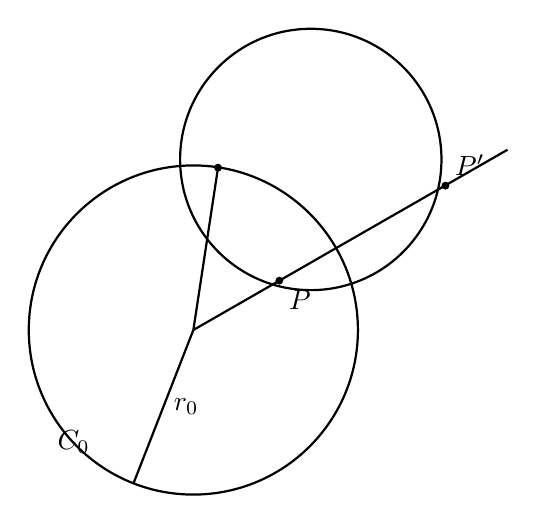
\begin{tikzpicture}[>=stealth, scale=0.95]
  \coordinate (O) at (0,0);
  \draw[thick] (O) circle (2.2cm);
  \node at (-1.6, -1.5) {$C_0$};
  
  % Radius r_0 drawn to lower-left
  \draw[thick] (O) -- (-0.8, -2.05) node[midway, right] {$r_0$};
  
  % Ray OPP' at 35 degrees
  \draw[thick] (O) -- (4.2, 2.41);
  
  \coordinate (P) at (1.15, 0.66);
  \coordinate (Pprime) at (3.37, 1.93);
  \fill (P) circle (1.5pt) node[below right] {$P$};
  \fill (Pprime) circle (1.5pt) node[above right] {$P'$};
  
  % Circle C through P, P' orthogonal to C_0
  % Midpoint of PP': (2.26, 1.30), normal (-0.5736, 0.8192)
  % Center: M + 1.2 * normal = (1.57, 2.28), R = sqrt(1.27^2 + 1.2^2) = 1.75
  \coordinate (K) at (1.57, 2.28);
  \draw[thick] (K) circle (1.747cm);
  
  % Tangent from O to C touches at intersection with C_0:
  % Tangent length = sqrt(KO^2 - R^2) = r_0 = 2.2!
  % Intersection T of C_0 and C
  \coordinate (T) at (0.33, 2.17);
  \draw[thick] (O) -- (T);
  \fill (T) circle (1.5pt);
\end{tikzpicture}
\caption{圓的鏡射：割線切線定理 $\overline{OP} \cdot \overline{OP'} = r_0^2$}
\label{fig:b4-3-40}
\end{figure}

\begin{proof}
設 $C$ 為任意一個過 $P$ 且與 $C_0$ 正交的圓，$P_0$ 為 $C$ 與 $C_0$ 的一個交點．設自原點 $O$ 引半射線 $OP$ 交 $C$ 於 $P$ 與 $P'$ 兩點．由圓的割線定理（線段長度乘積定理）：
\[ \overline{OP} \cdot \overline{OP'} = \overline{OP_0}^2 = r_0^2 \]
因 $P$ 之座標為 $(a,b)$，其長度 $\overline{OP} = \sqrt{a^2 + b^2}$，故
\[ \overline{OP'} = \frac{r_0^2}{\sqrt{a^2 + b^2}} \]
因 $P'$ 落在射線 $OP$ 上，若設 $P' = (\lambda a, \lambda b)$，則
\[ \lambda = \frac{\overline{OP'}}{\overline{OP}} = \frac{r_0^2}{a^2 + b^2} \]
因此 $P'$ 之座標為
\[ P' = \left(\frac{r_0^2 a}{a^2 + b^2}, \frac{r_0^2 b}{a^2 + b^2}\right) \]
容易看出上式只與圓 $C_0$ 的半徑 $r_0$ 及 $P$ 的座標 $a, b$ 有關，而不因圓 $C$ 之選取不同而受影響！換句話說，所有過 $P$ 且正交於 $C_0$ 的圓皆通過 $P'$ 點，故 $P'$ 為 $P$ 之 $C_0$-鏡像點．
\end{proof}

因為過點 $P$ 且與圓 $C_0$ 正交的圓均過另一點 $P'$，而過二點 $P$ 與 $P'$ 的圓的圓心皆在線段 $PP'$ 的垂直平分線上，故知圓 $C$ 所做成集合的自由度為 1（等於 $PP'$ 垂直平分線的自由度），我們稱此圓的集合為一\textbf{圓系}．

\begin{figure}[htbp]
\centering
\begin{tikzpicture}[>=stealth, scale=0.95]
  \coordinate (O) at (0,0);
  \draw[thick] (O) circle (2.2cm);
  \node[below] at (0, -2.3) {$C_0$};
  
  % Ray through P and P'
  \draw[thick] (-0.5, -0.29) -- (4.3, 2.47);
  
  \coordinate (P) at (1.15, 0.66);
  \coordinate (Pprime) at (3.37, 1.93);
  \fill (P) circle (1.5pt) node[below right] {$P$};
  \fill (Pprime) circle (1.5pt) node[above right] {$P'$};
  
  % Perpendicular bisector line of PP'
  % Midpoint M = (2.26, 1.30), normal vector n = (-0.5736, 0.8192)
  \draw[thick] ($(2.26, 1.30) - 2.8*(-0.5736, 0.8192)$) -- ($(2.26, 1.30) + 3.2*(-0.5736, 0.8192)$);
  
  % Family of circles passing through P and P' with centers on the bisector
  % Circle 1: h = 1.4 -> Center = M + 1.4*n = (1.46, 2.45), R = sqrt(1.27^2 + 1.4^2) = 1.89
  \draw[thick] (1.46, 2.45) circle (1.89cm);
  % Circle 2: h = 0.5 -> Center = M + 0.5*n = (1.97, 1.71), R = sqrt(1.27^2 + 0.5^2) = 1.36
  \draw[thick] (1.97, 1.71) circle (1.36cm);
  % Circle 3: h = -1.5 -> Center = M - 1.5*n = (3.12, 0.07), R = sqrt(1.27^2 + 1.5^2) = 1.96
  \draw[thick] (3.12, 0.07) circle (1.96cm);
\end{tikzpicture}
\caption{同軸圓系：所有過 $P$ 且正交於 $C_0$ 的圓皆過鏡像點 $P'$}
\label{fig:b4-3-41}
\end{figure}

\begin{theorem}
對於圓的鏡射把不通過原點的圓帶到圓．
\end{theorem}

\begin{proof}
設 $C_0 : x^2 + y^2 = r_0^2$ 為鏡射圈，$f$ 為 $C_0$-鏡射．\\
設 $C : x^2 + y^2 + 2Dx + 2Ey + F = 0$ ($F \neq 0$，卽不通過原點）為一圓．\\
當 $P(a,b) \in C$ 時，設其鏡像點 $P' = f(P)$ 之座標為 $(a', b')$．\\
由對稱性，$P$ 亦為 $P'$ 之 $C_0$-鏡像點，故
\[ a = \frac{r_0^2 a'}{a'^2 + b'^2}, \qquad b = \frac{r_0^2 b'}{a'^2 + b'^2} \]
將 $(a,b)$ 代入 $C$ 的方程式得
\[ \left(\frac{r_0^2 a'}{a'^2 + b'^2}\right)^2 + \left(\frac{r_0^2 b'}{a'^2 + b'^2}\right)^2 + 2D\left(\frac{r_0^2 a'}{a'^2 + b'^2}\right) + 2E\left(\frac{r_0^2 b'}{a'^2 + b'^2}\right) + F = 0 \]
展開整理得
\[ \frac{r_0^4}{(a'^2 + b'^2)} + 2Dr_0^2 a' + 2Er_0^2 b' + F(a'^2 + b'^2) = 0 \]
兩邊同乘以 $(a'^2 + b'^2)$ 後除以 $F$（因 $F \neq 0$）：
\[ a'^2 + b'^2 + \frac{2Dr_0^2}{F}a' + \frac{2Er_0^2}{F}b' + \frac{r_0^4}{F} = 0 \]
此式為圓 $C$ 的鏡像曲線 $f(C)$ 的軌跡方程式，顯然仍為一圓！
\end{proof}

\begin{exercise}
\begin{enumerate}[(i)]
  \item 若 $P$ 點在圓 $C_0$ 內，則其 $C_0$-鏡像點在圓外；若 $P$ 在圓 $C_0$ 上，則其鏡像點為自身．
  \item 試求點 $(\frac{1}{2}, \frac{1}{2})$ 對於單位圓的鏡像點．
\end{enumerate}
\end{exercise}

\subsubsection*{習題 III-6}

\begin{enumerate}
  \item 求二圓 $x^2 + y^2 = 16$ 及 $x^2 - 10x + y^2 + 16 = 0$ 之交點與交角．\\
  （提示：求交角可用切線向量或法線向量之內積）

  \item 求與二圓 $(x-1)^2 + (y-2)^2 = 20$ 及 $x^2 + y^2 = 25$ 相切並過點 $(13, 4)$ 的圓方程式．

  \item 求過 $(-1, 9)$ 及 $(-5, -1)$ 兩點並與圓 $(x-3)^2 + (y+4)^2 = 25$ 相切的圓．

  \item 試討論二圓
  \begin{align*}
  x^2 + y^2 + 2D_1x + 2E_1y + F_1 &= 0 \\
  x^2 + y^2 + 2D_2x + 2E_2y + F_2 &= 0
  \end{align*}
  相交，相切或相離的條件為
  \[ \left(D_1D_2 + E_1E_2 - \frac{F_1 + F_2}{2}\right)^2 - (D_1^2 + E_1^2 - F_1)(D_2^2 + E_2^2 - F_2) \]
  小於，等於或大於零．
\end{enumerate}
